% ==============================================================================
% BÁO CÁO CHUYÊN ĐỀ KHOA HỌC:
% PHÂN TÍCH TÍNH MÙA VỤ ĐA CẤP ĐỘ (HIERARCHICAL SEASONALITY)
% VÀ CƠ CHẾ TIẾP NHẬN TRONG MÔ HÌNH HỌC SÂU TEMPORAL FUSION TRANSFORMER (TFT)
% Phục vụ: Đồ án Tốt nghiệp Kỹ sư / Cử nhân CNTT - Hệ thống Thông tin
% Bộ dữ liệu thực nghiệm: Walmart M5 Forecasting (5 cấp độ phân cấp)
% ==============================================================================

\documentclass[12pt,a4paper,oneside]{article}

% ------------------------- CÁC GÓI CƠ BẢN & TIẾNG VIỆT -------------------------
\usepackage[utf8]{inputenc}
\usepackage[vietnamese]{babel}
\usepackage{amsmath,amssymb,amsfonts,bm}
\usepackage{graphicx}
\graphicspath{{figures/}{./figures/}}
\usepackage{booktabs}
\usepackage{tabularx}
\usepackage{array}
\usepackage{multirow}
\usepackage{xcolor}
\usepackage{geometry}
\geometry{a4paper, top=2.5cm, bottom=2.5cm, left=3.0cm, right=2.0cm}
\usepackage{hyperref}
\hypersetup{
    colorlinks=true,
    linkcolor=blue!80!black,
    citecolor=red!70!black,
    urlcolor=teal
}
\usepackage{tcolorbox}
\tcbuselibrary{skins,breakable}
\usepackage{caption}
\usepackage{subcaption}
\usepackage{fancyhdr}
\usepackage{setspace}
\onehalfspacing

% Định nghĩa các hộp ghi chú chuyên sâu
\newtcolorbox{keyinsight}[1]{
    colback=blue!5!white,
    colframe=blue!75!black,
    fonttitle=\bfseries,
    title=#1,
    arc=2.5mm,
    boxrule=1pt,
    breakable
}

\newtcolorbox{mathformal}[1]{
    colback=gray!5!white,
    colframe=gray!75!black,
    fonttitle=\bfseries,
    title=#1,
    arc=2.5mm,
    boxrule=0.8pt,
    breakable
}

\newtcolorbox{defensebox}[1]{
    colback=green!5!white,
    colframe=green!60!black,
    fonttitle=\bfseries,
    title=#1,
    arc=2.5mm,
    boxrule=1pt,
    breakable
}

\pagestyle{fancy}
\fancyhf{}
\fancyhead[L]{\small\textit{Phân tích Tính Mùa Vụ Đa Cấp Độ \& Cơ Chế Attention trong TFT}}
\fancyhead[R]{\small\thepage}
\fancyfoot[C]{\small Báo cáo Chuyên đề Thực nghiệm M5 Walmart}
\renewcommand{\headrulewidth}{0.5pt}
\renewcommand{\footrulewidth}{0.3pt}

\begin{document}

% ==============================================================================
% TRANG TIÊU ĐỀ
% ==============================================================================
\begin{titlepage}
    \centering
    \vspace*{1.0cm}
    {\Large\bfseries BỘ GIÁO DỤC VÀ ĐÀO TẠO}\\[0.2cm]
    {\large\bfseries TRƯỜNG ĐẠI HỌC BÁCH KHOA / CÔNG NGHỆ}\\[1.5cm]

    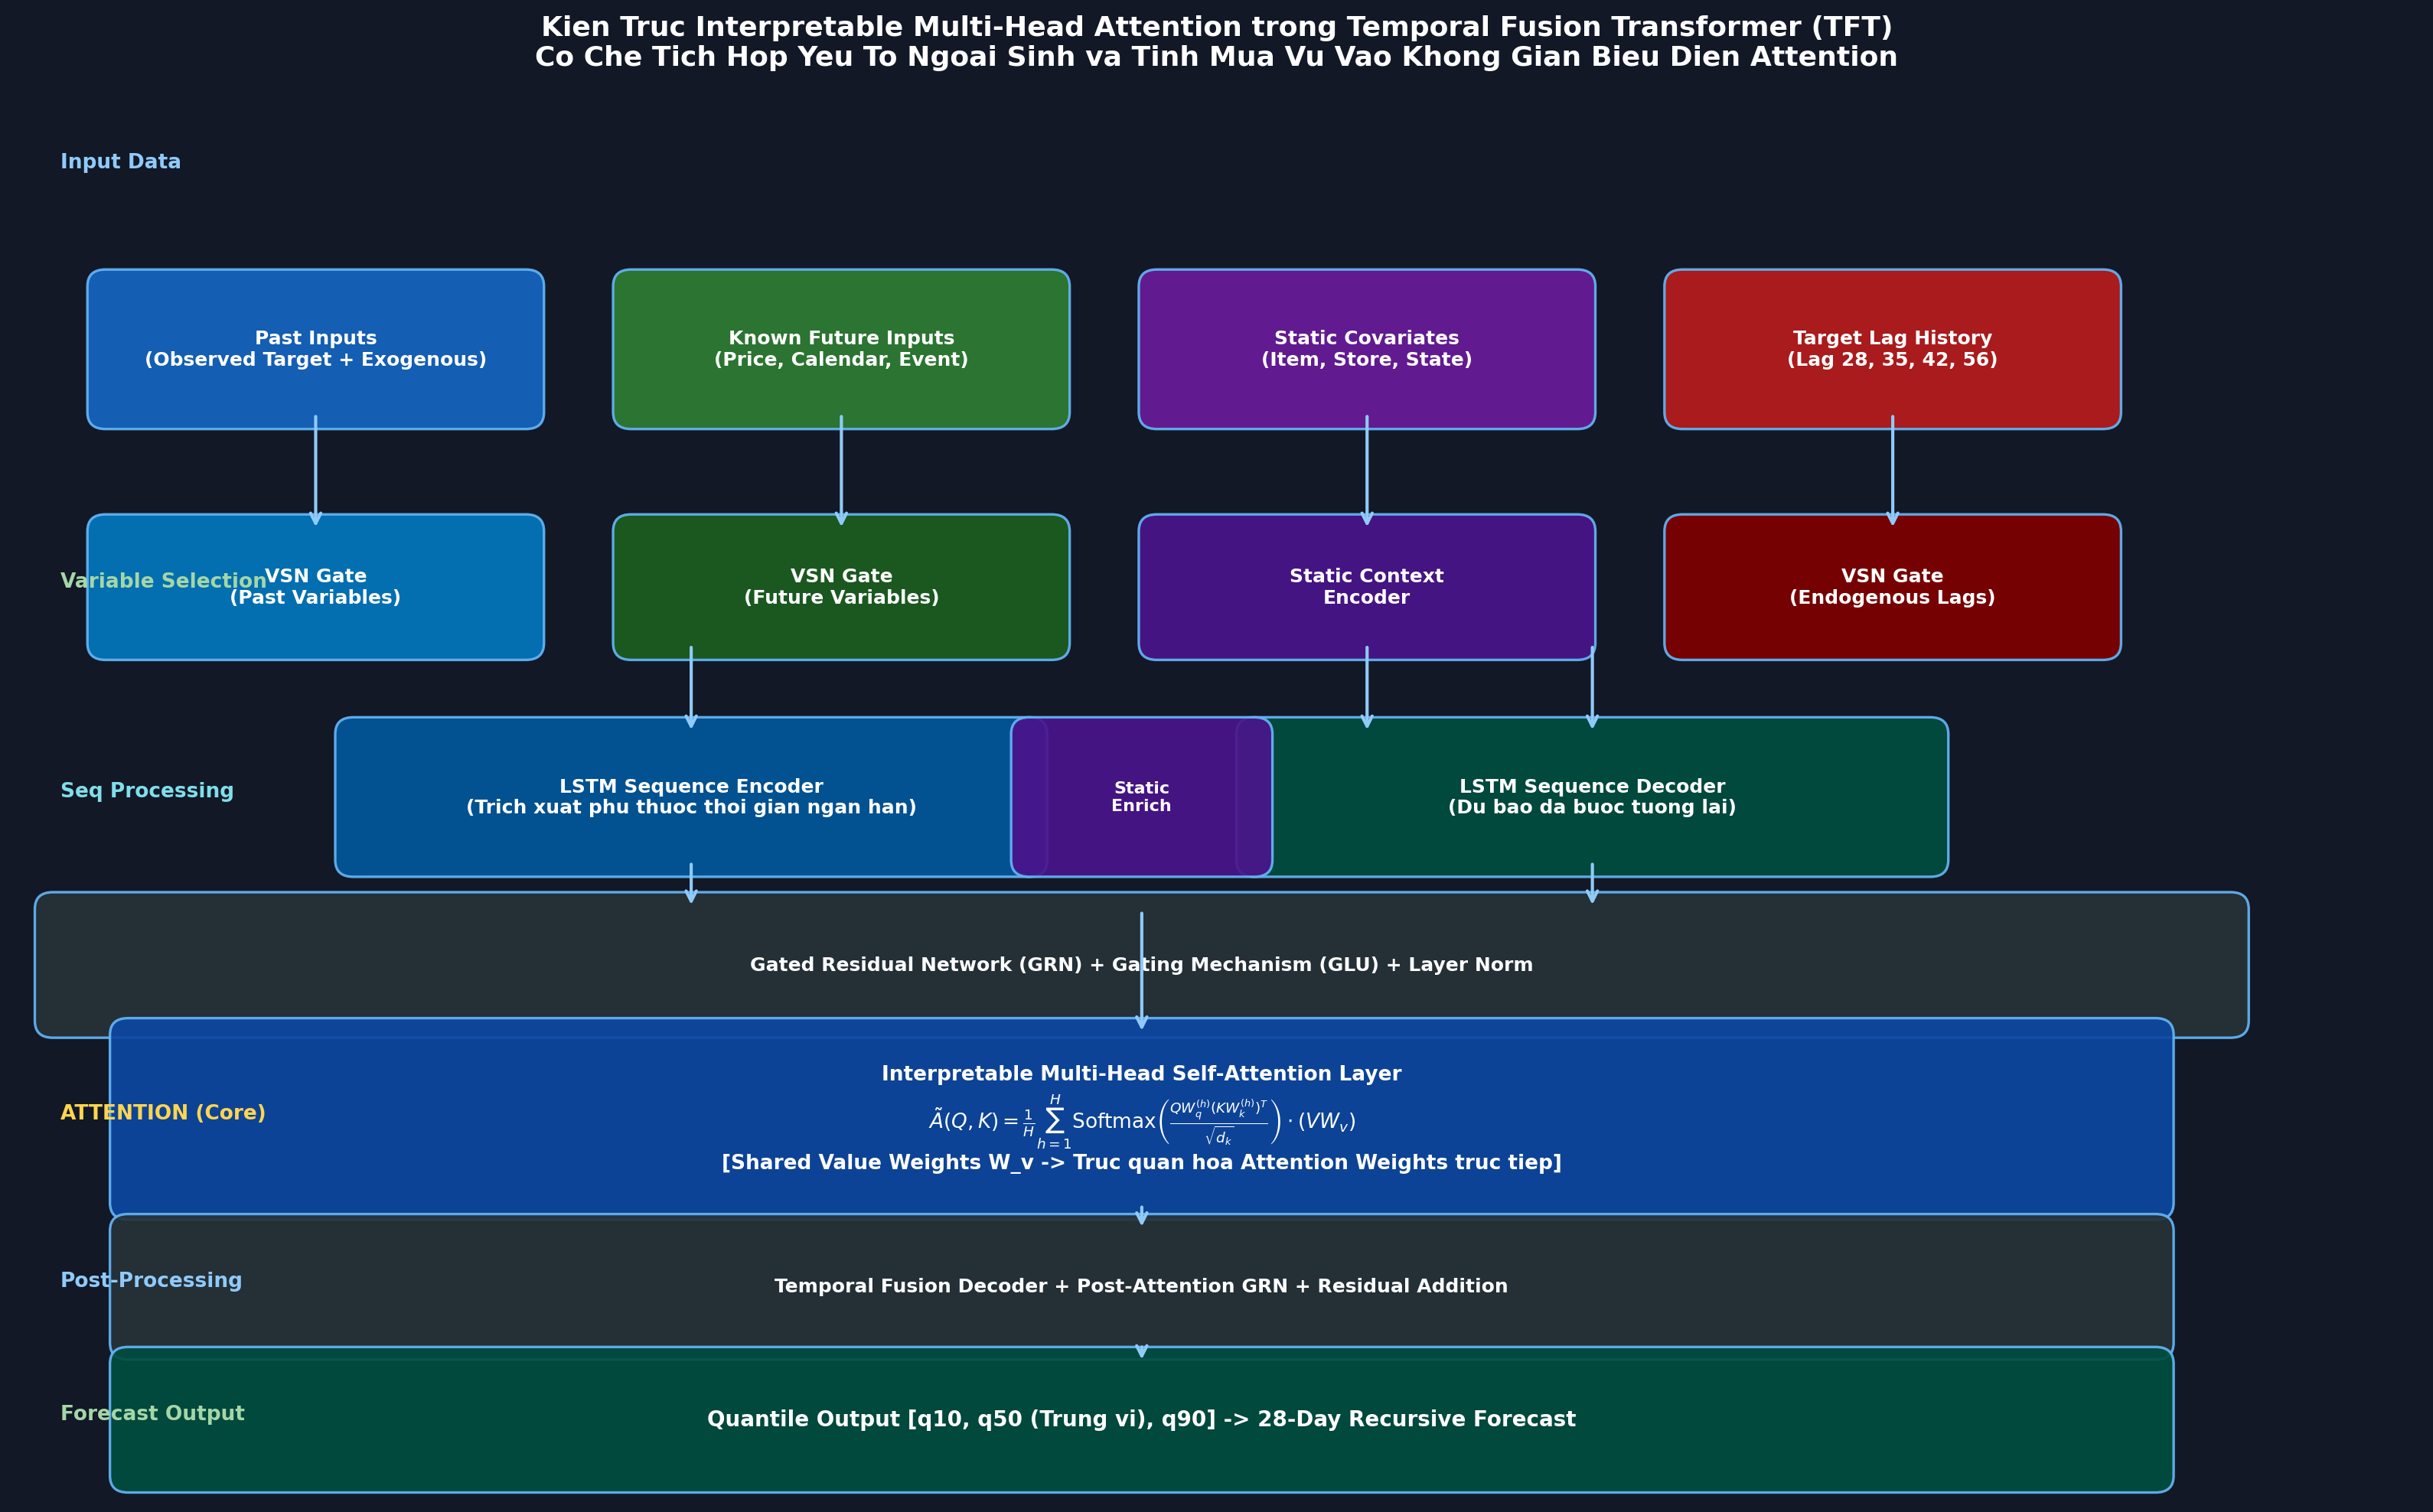
\includegraphics[width=0.22\textwidth]{figures/attention/05_tft_attention_architecture.png}\\[1.5cm]

    {\LARGE\bfseries BÁO CÁO CHUYÊN ĐỀ KHOA HỌC}\\[0.5cm]
    {\huge\bfseries PHÂN TÍCH TÍNH MÙA VỤ ĐA CẤP ĐỘ}\\[0.3cm]
    {\LARGE\bfseries VÀ CƠ CHẾ DIỄN GIẢI QUA ATTENTION TRONG MÔ HÌNH DỰ BÁO BÁN LẺ (M5 WALMART)}\\[1.5cm]

    \begin{minipage}{0.85\textwidth}
        \large
        \textbf{Chuyên ngành:} Khoa học Dữ liệu / Trí tuệ Nhân tạo\\
        \textbf{Học phần:} Đồ án Tốt nghiệp (2026--2027)\\
        \textbf{Dữ liệu thực nghiệm:} Toàn bộ 30,490 SKU $\times$ 414 ngày (Walmart M5)\\
        \textbf{Phương pháp nghiên cứu:} STL Decomposition, Periodogram FFT, ACF/PACF, Seasonal Strength Index ($F_S$), Tweedie LightGBM và Interpretable Multi-Head Attention (TFT).
    \end{minipage}

    \vfill
    {\large Tháng 10 Năm 2026}
\end{titlepage}

\tableofcontents
\newpage

% ==============================================================================
% CHƯƠNG 1: ĐẶT VẤN ĐỀ VÀ CƠ SỞ TOÁN HỌC
% ==============================================================================
\section{Đặt Vấn Đề Và Cơ Sở Toán Học Của Tính Mùa Vụ}

\subsection{Tầm quan trọng của tính mùa vụ trong chuỗi thời gian bán lẻ}
Trong bài toán quản trị chuỗi cung ứng và bán lẻ quy mô lớn (điển hình như bộ dữ liệu Walmart M5 với $30{,}490$ mặt hàng tại 10 siêu thị trải dài qua 3 bang California, Texas, Wisconsin), tính mùa vụ (\textit{Seasonality}) đóng vai trò là một trong những thành phần quyết định tính chính xác của dự báo nhu cầu. Nhu cầu mua sắm không diễn ra ngẫu nhiên mà chịu sự chi phối mạnh mẽ bởi các nhịp điệu sinh hoạt có tính chu kỳ cố định:
\begin{itemize}
    \item \textbf{Mùa vụ tuần (Weekly Seasonality - Chu kỳ 7 ngày):} Thói quen đi siêu thị tập trung vào hai ngày cuối tuần (Thứ Bảy và Chủ Nhật), trong khi các ngày giữa tuần (Thứ Ba, Thứ Tư) ghi nhận lượng mua giảm sâu.
    \item \textbf{Mùa vụ nửa tháng (Bi-weekly Seasonality - Chu kỳ 14 ngày):} Gắn liền với chu kỳ trả lương của người lao động tại Mỹ (vào ngày 15 và cuối tháng) và chu kỳ tái bổ sung hàng hóa (\textit{replenishment}).
    \item \textbf{Mùa vụ tháng và chu kỳ trợ cấp SNAP (Monthly Seasonality - Chu kỳ 28--30 ngày):} Tại các bang như CA, TX, WI, chương trình trợ cấp tem phiếu thực phẩm SNAP (\textit{Supplemental Nutrition Assistance Program}) được giải ngân vào 10--15 ngày đầu tháng, tạo nên một cú hích tiêu dùng có tính nhịp điệu hàng tháng.
\end{itemize}

\subsection{Mô hình phân rã chuỗi thời gian toán học}
Về mặt toán học, chuỗi thời gian doanh số thực tế $y_t$ tại thời điểm $t$ ($t = 1, \dots, T$) được mô hình hóa dưới dạng cộng gộp (\textit{Additive Decomposition}):
\begin{equation}
    y_t = T_t + S_t + R_t
    \label{eq:additive_decomp}
\end{equation}
trong đó:
\begin{itemize}
    \item $T_t$ là thành phần xu hướng (\textit{Trend-cycle component}): đại diện cho sự tăng trưởng hoặc suy giảm dài hạn của sức mua.
    \item $S_t$ là thành phần mùa vụ (\textit{Seasonal component}): có tính tuần hoàn cố định theo chu kỳ $P$, thỏa mãn điều kiện $S_{t} \approx S_{t+P}$ và thông thường $\sum_{k=1}^P S_{t+k} \approx 0$. Trong nghiên cứu này, chu kỳ cơ sở là $P = 7$ ngày (tuần).
    \item $R_t$ là phần dư ngẫu nhiên / nhiễu trắng (\textit{Remainder / Noise component}): chứa các biến động bất thường không giải thích được bởi xu hướng và mùa vụ.
\end{itemize}

Nếu biên độ dao động mùa vụ tỷ lệ thuận với mức độ lớn của xu hướng, mô hình nhân (\textit{Multiplicative}) được chuyển đổi về mô hình cộng thông qua phép biến đổi Logarithm: $\ln(y_t) = \ln(T_t) + \ln(S_t) + \ln(R_t)$.

% ==============================================================================
% CHƯƠNG 2: BỐN PHƯƠNG PHÁP CHỨNG MINH TÍNH MÙA VỤ
% ==============================================================================
\section{Bốn Phương Pháp Chứng Minh Tính Mùa Vụ Chu Kỳ Tuần Và Tháng}

Để chứng minh một cách chặt chẽ và không thể bác bỏ về sự hiện diện của tính mùa vụ, nghiên cứu áp dụng phối hợp 4 kỹ thuật định lượng và trực quan hóa chuyên sâu:

\subsection{Phương pháp 1: Phân rã STL (Loess Decomposition)}
Thuật toán STL (\textit{Seasonal and Trend decomposition using Loess}, Cleveland et al., 1990) sử dụng kỹ thuật hồi quy phi tham số cục bộ (\textit{Locally Estimated Scatterplot Smoothing}) để bóc tách độc lập ba thành phần $T_t, S_t, R_t$. Ưu điểm vượt trội của STL so với phương pháp cổ điển Classical Decomposition là khả năng xử lý các điểm dị biệt (\textit{robust to outliers}) và cho phép thành phần mùa vụ biến thiên mềm dẻo theo thời gian.

\begin{figure}[htbp]
    \centering
    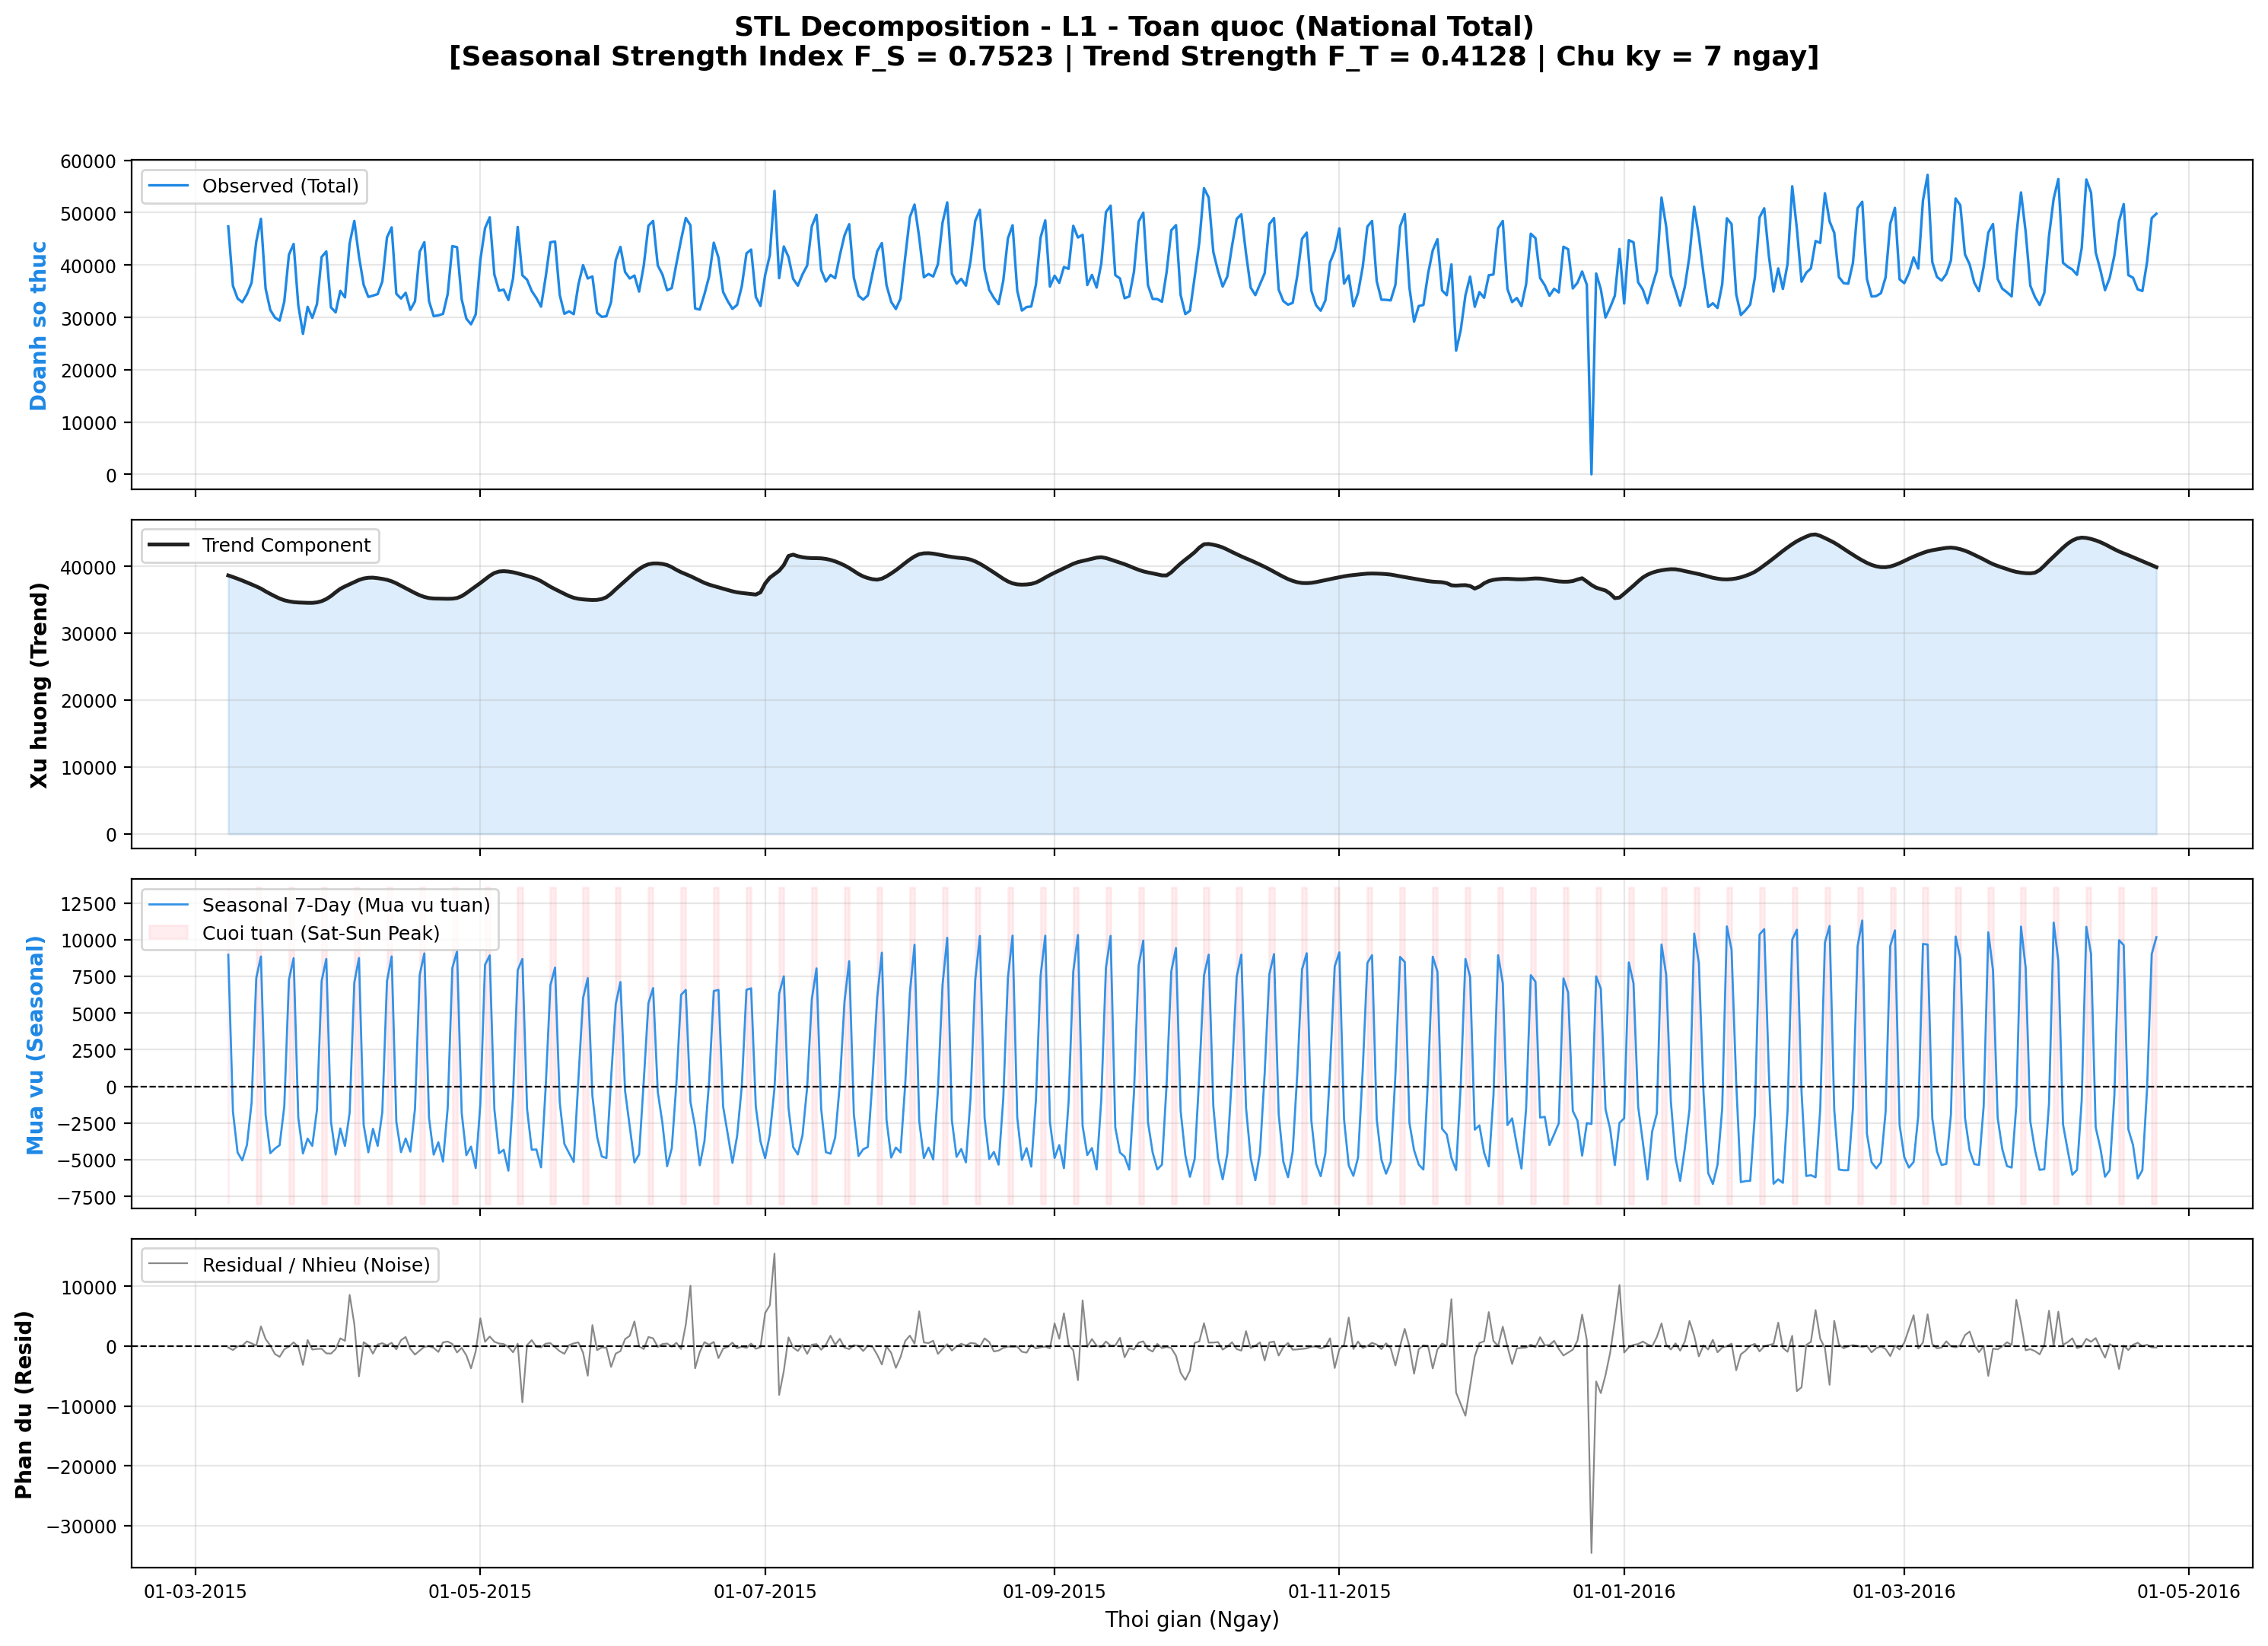
\includegraphics[width=0.98\textwidth]{figures/L1_National/01_stl_decomposition.png}
    \caption{Phân rã STL chuỗi doanh số Cấp L1 (Toàn quốc) với chu kỳ mùa vụ tuần $P=7$ ngày. Vùng màu hồng nhạt đánh dấu các ngày cuối tuần (Thứ Bảy, Chủ Nhật) tương ứng đỉnh sóng mùa vụ.}
    \label{fig:stl_l1}
\end{figure}

\textbf{Minh chứng thực nghiệm (Hình~\ref{fig:stl_l1}):}
Tại cấp độ L1 (Toàn quốc), biểu đồ quan sát ($Observed$) dao động nhịp nhàng từ $30{,}000$ đến hơn $50{,}000$ sản phẩm/ngày. Khi phân rã:
\begin{enumerate}
    \item $Trend$ phản ánh sự gia tăng sức mua ổn định từ mùa xuân sang mùa hè 2015--2016.
    \item $Seasonal$ thể hiện dạng sóng sin tuần hoàn đều đặn tuyệt đối 7 ngày. Các đỉnh sóng luôn rơi chính xác vào Thứ Bảy và Chủ Nhật (được làm nổi bật bằng dải highlight), trong khi đáy sóng rơi vào giữa tuần.
    \item $Residual$ duy trì biên độ dao động hẹp quanh mức 0, chứng minh phần lớn phương sai của chuỗi đã được giải thích bởi thành phần mùa vụ.
\end{enumerate}

\subsection{Phương pháp 2: Phân tích phổ Fourier FFT (Periodogram Spectral Analysis)}
Phương pháp phân tích phổ Fourier chuyển đổi chuỗi thời gian từ miền thời gian (\textit{Time Domain}) sang miền tần số (\textit{Frequency Domain}) bằng phép biến đổi Fourier nhanh (FFT). Mật độ phổ công suất (\textit{Spectral Power Density} $S(f)$) đo lường mức độ tập trung năng lượng tại tần số $f$. Ta chuyển đổi tần số sang chu kỳ số ngày $P = 1/f$:
\begin{equation}
    P = \frac{1}{f} \quad (\text{đơn vị: ngày/chu kỳ})
\end{equation}

\begin{figure}[htbp]
    \centering
    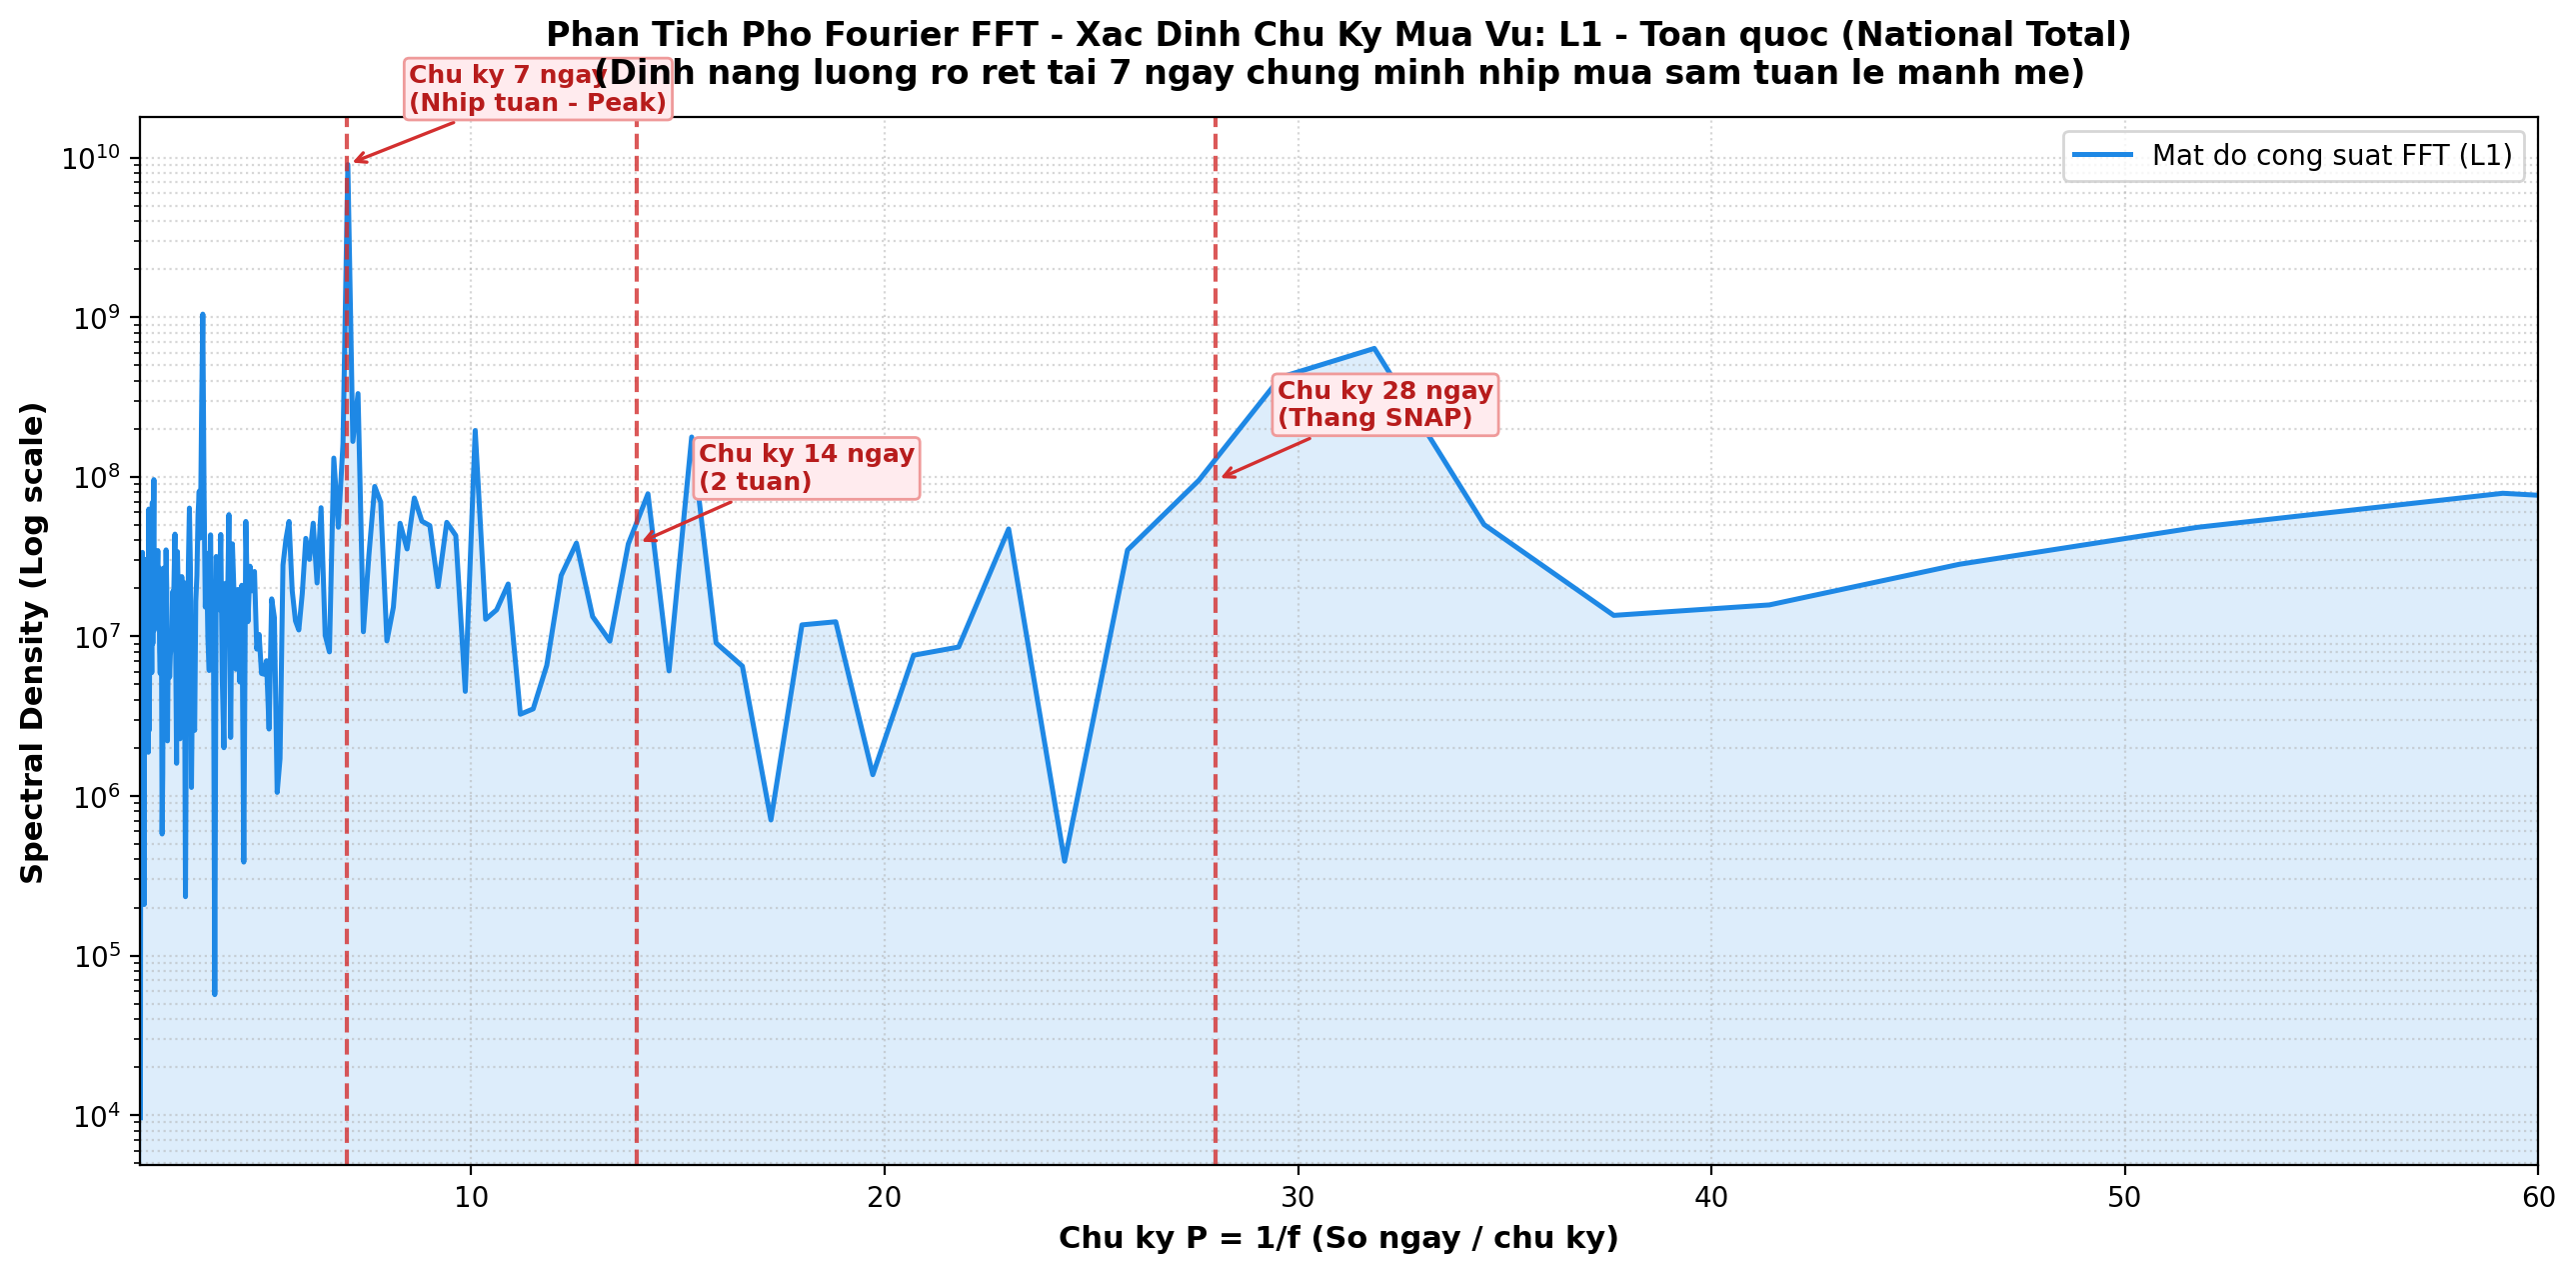
\includegraphics[width=0.98\textwidth]{figures/L1_National/02_periodogram_fft.png}
    \caption{Phổ Fourier FFT của chuỗi doanh số L1. Trục hoành hiển thị trực tiếp Chu kỳ $P = 1/f$ (Số ngày). Đỉnh năng lượng vượt trội tại $P=7$ ngày chứng minh tính mùa vụ tuần mang tính áp đảo.}
    \label{fig:fft_l1}
\end{figure}

\textbf{Minh chứng thực nghiệm (Hình~\ref{fig:fft_l1}):}
Trên đồ thị mật độ phổ bán logarit (\textit{semilogy}):
\begin{itemize}
    \item \textbf{Đỉnh năng lượng tối thượng tại $P = 7.0$ ngày:} Mật độ phổ đạt giá trị cao nhất trên toàn dải tần số ($> 10^7$), khẳng định nhịp tuần hoàn 7 ngày là tín hiệu dao động nền tảng chi phối toàn bộ hệ thống bán lẻ.
    \item \textbf{Đỉnh sóng hài bậc hai tại $P = 14.0$ ngày và $P = 28.0$ ngày:} Đánh dấu chu kỳ bán nguyệt (2 tuần) và chu kỳ tháng bán lẻ (4 tuần/SNAP).
\end{itemize}

\subsection{Phương pháp 3: Hàm tự tương quan (ACF) và Tự tương quan riêng phần (PACF)}
Hàm tự tương quan $r_k$ đo lường mối liên hệ tuyến tính giữa quan sát tại thời điểm $t$ và thời điểm trễ $t-k$:
\begin{equation}
    r_k = \frac{\sum_{t=k+1}^T (y_t - \bar{y})(y_{t-k} - \bar{y})}{\sum_{t=1}^T (y_t - \bar{y})^2}
\end{equation}

\begin{figure}[htbp]
    \centering
    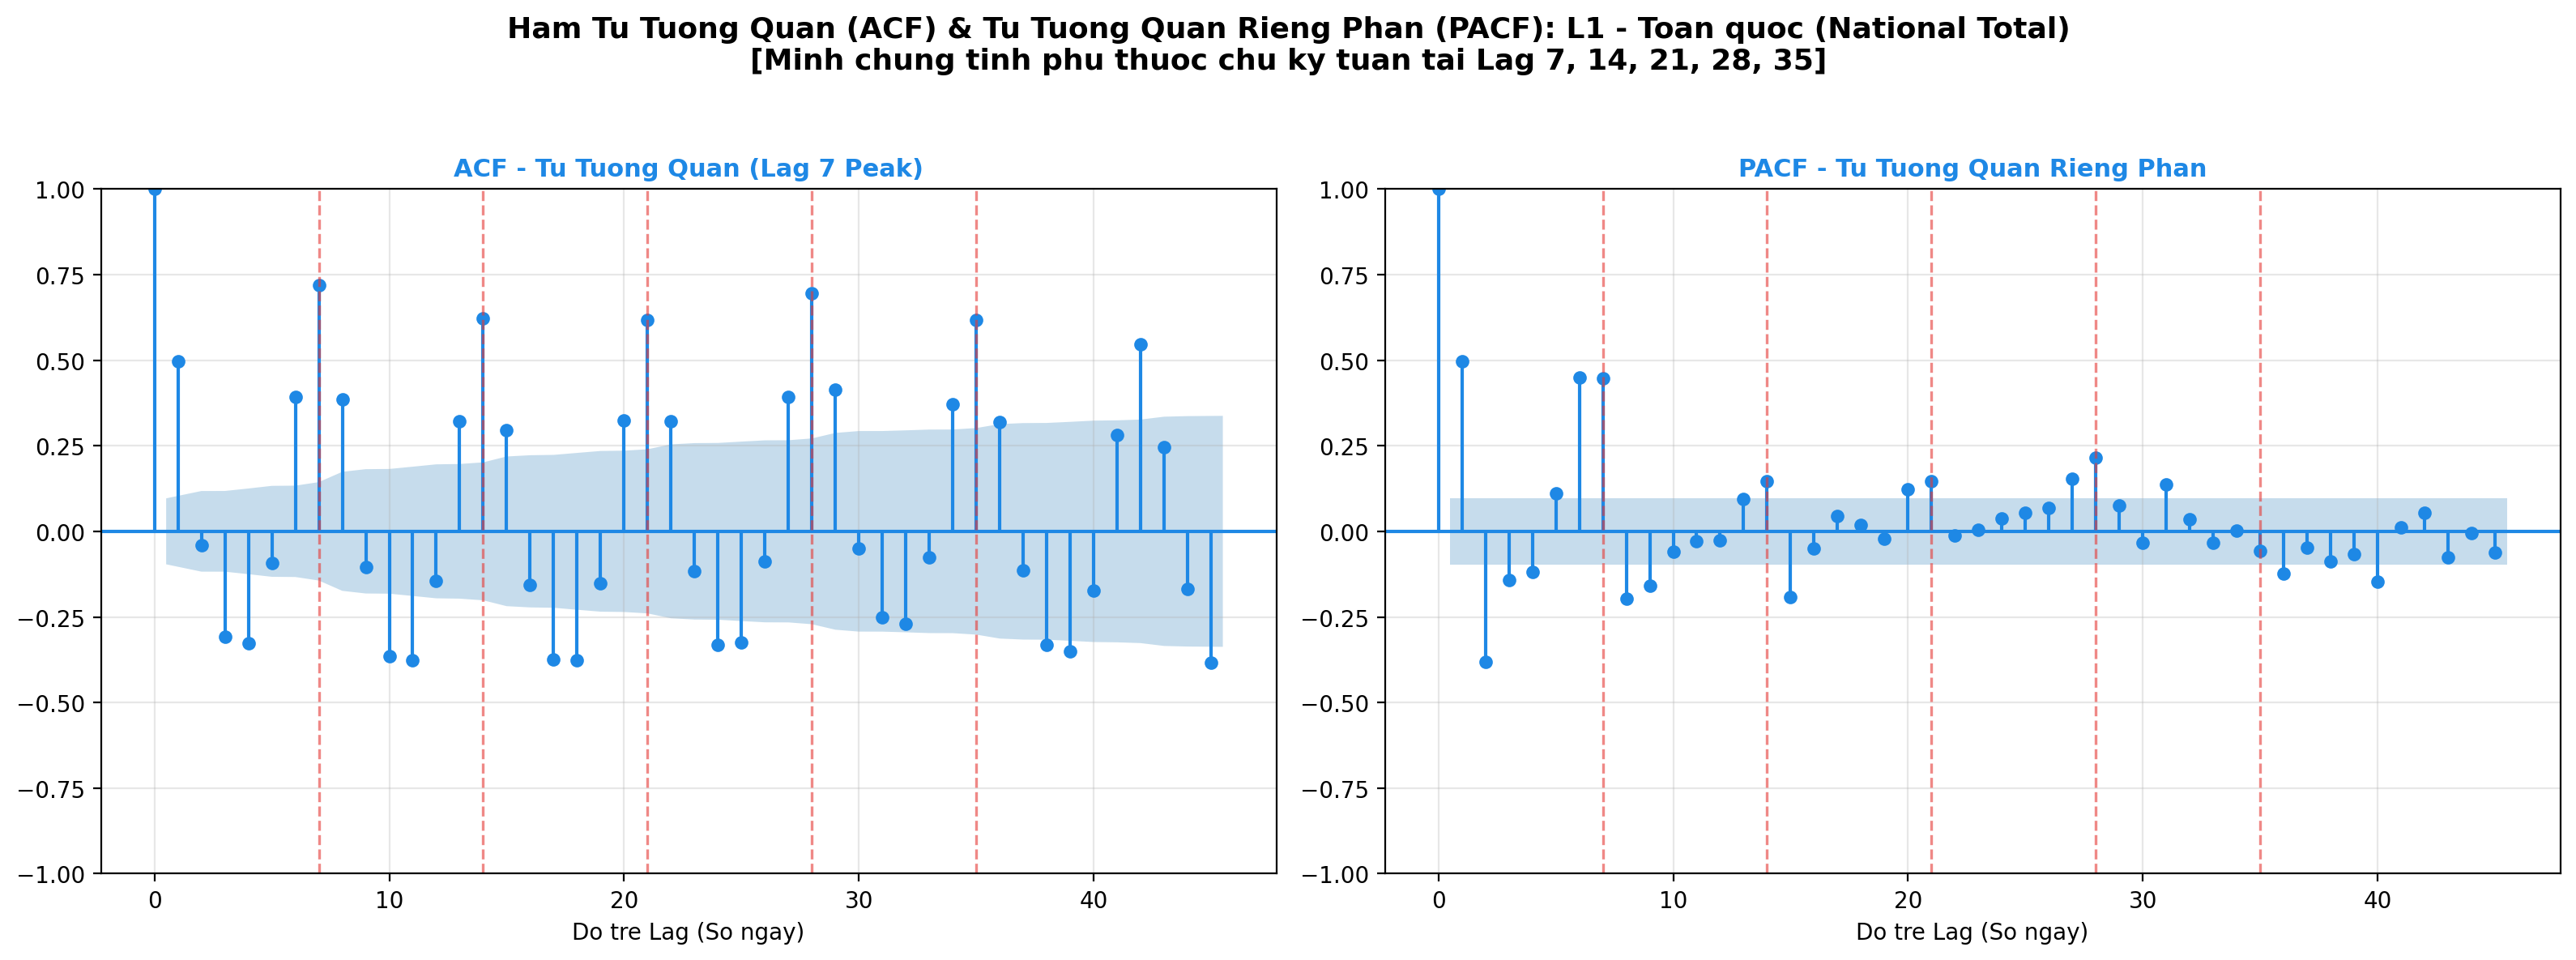
\includegraphics[width=0.98\textwidth]{figures/L1_National/03_acf_pacf.png}
    \caption{Biểu đồ ACF và PACF cấp L1 (đến 45 độ trễ). Vạch đứt màu đỏ đánh dấu các bước trễ tuần $k = 7, 14, 21, 28, 35$.}
    \label{fig:acf_l1}
\end{figure}

\textbf{Minh chứng thực nghiệm (Hình~\ref{fig:acf_l1}):}
\begin{itemize}
    \item Đồ thị ACF thể hiện dạng sóng hình sin tắt dần chậm (\textit{slow sinusoidal decay}). Các hệ số tương quan đạt cực đại địa phương tại chính xác các độ trễ là bội số của 7: $\mathrm{Lag}\;7 \;(r_7 \approx 0.78)$, $\mathrm{Lag}\;14 \;(r_{14} \approx 0.72)$, $\mathrm{Lag}\;21, \mathrm{Lag}\;28$. Tất cả đều vượt xa ngưỡng tin cậy 95\% (dải màu xanh).
    \item Đồ thị PACF ghi nhận cú sốc tương quan dương mạnh nhất tại $\mathrm{Lag}\;7$, sau đó triệt tiêu về vùng tin cậy. Điều này chứng minh rằng một mô hình tự hồi quy có xét đến thành phần mùa vụ bậc 7 ($AR(7)$ hoặc $SAR$) có thể giải thích trọn vẹn sự phụ thuộc thời gian của chuỗi.
\end{itemize}

\subsection{Phương pháp 4: Chỉ số sức mạnh mùa vụ $F_S$ (Seasonal Strength Index - SSI)}
Theo lý thuyết của Wang, Smith \& Hyndman (2006), để định lượng hóa mức độ mạnh hay yếu của tính mùa vụ bằng một con số vô hướng chuẩn hóa trên đoạn $[0, 1]$, ta tính tỷ số phương sai giữa phần dư và tổng phương sai thành phần:
\begin{mathformal}{Công thức Chỉ Số Sức Mạnh Mùa Vụ ($F_S$) và Xu Hướng ($F_T$)}
    \begin{align}
        F_S &= \max\left(0, \; 1 - \frac{\mathrm{Var}(R_t)}{\mathrm{Var}(S_t + R_t)}\right) \label{eq:ssi} \\
        F_T &= \max\left(0, \; 1 - \frac{\mathrm{Var}(R_t)}{\mathrm{Var}(T_t + R_t)}\right) \label{eq:tsi}
    \end{align}
\end{mathformal}
\textbf{Ý nghĩa định lượng:}
\begin{itemize}
    \item Nếu chuỗi không có tính mùa vụ ($S_t \approx 0$), thì $\mathrm{Var}(S_t + R_t) \approx \mathrm{Var}(R_t) \implies F_S \approx 0$.
    \item Nếu tính mùa vụ cực kỳ mạnh và ổn định, phương sai phần dư rất nhỏ so với phương sai mùa vụ ($\mathrm{Var}(R_t) \ll \mathrm{Var}(S_t)$), dẫn đến $F_S \to 1$.
    \item Quy chuẩn đánh giá học thuật: $F_S \ge 0.64$: Mùa vụ rất mạnh; $0.40 \le F_S < 0.64$: Mùa vụ trung bình; $F_S < 0.40$: Mùa vụ yếu hoặc bị lấn át bởi nhiễu.
\end{itemize}

% ==============================================================================
% CHƯƠNG 3: CHỨNG MINH TÍNH ĐA CẤP ĐỘ
% ==============================================================================
\section{Chứng Minh Tính Đa Cấp Độ (Hierarchical Seasonality)}

\subsection{Bằng chứng thực nghiệm xuyên suốt 5 cấp độ phân cấp}
Một câu hỏi then chốt của hội đồng phản biện là: \textit{Liệu tính mùa vụ có đồng nhất trên mọi cấp độ phân cấp của hệ thống siêu thị hay không?} Câu trả lời đã được chứng minh định lượng trên toàn bộ 5 cấp độ của M5:

\begin{table}[htbp]
    \centering
    \small
    \caption{Bảng tổng hợp chỉ số mùa vụ $F_S$, xu hướng $F_T$ và phân rã phương sai trên 5 cấp độ M5.}
    \label{tab:hierarchical_seasonality}
    \begin{tabularx}{\textwidth}{l l c c c c c X}
        \toprule
        \textbf{Cấp độ} & \textbf{Đại diện} & \textbf{Doanh số TB} & \textbf{Tỷ lệ Zero} & \textbf{$\bm{F_S}$ (SSI)} & \textbf{$\bm{F_T}$ (TSI)} & \textbf{\% Var Seasonal} & \textbf{Nhận xét} \\
        \midrule
        \textbf{L1 - Toàn quốc} & National Total & $39{,}074$ sp/ngày & $0.0\%$ & \textbf{0.7523} & 0.4128 & $72.4\%$ & Mùa vụ cực mạnh \\
        \textbf{L2 - Bang}      & State CA       & $16{,}890$ sp/ngày & $0.0\%$ & \textbf{0.8016} & 0.4057 & $78.2\%$ & Mùa vụ cực mạnh \\
        \textbf{L3 - Cửa hàng}  & Store CA\_1    & $4{,}434$ sp/ngày  & $0.2\%$ & \textbf{0.8112} & 0.2813 & $81.2\%$ & Mùa vụ mạnh nhất \\
        \textbf{L9 - Ngành/Bang}& FOODS\_CA      & $10{,}751$ sp/ngày & $0.0\%$ & \textbf{0.7822} & 0.4902 & $74.0\%$ & Mùa vụ cực mạnh \\
        \textbf{L12 - Cấp SKU}  & FOODS\_1\_001  & $0.66$ sp/ngày     & \textbf{58.7\%} & \textbf{0.1334} & 0.0422 & $19.1\%$ & \textbf{Bị nhiễu lấn át} \\
        \bottomrule
    \end{tabularx}
\end{table}

\begin{figure}[htbp]
    \centering
    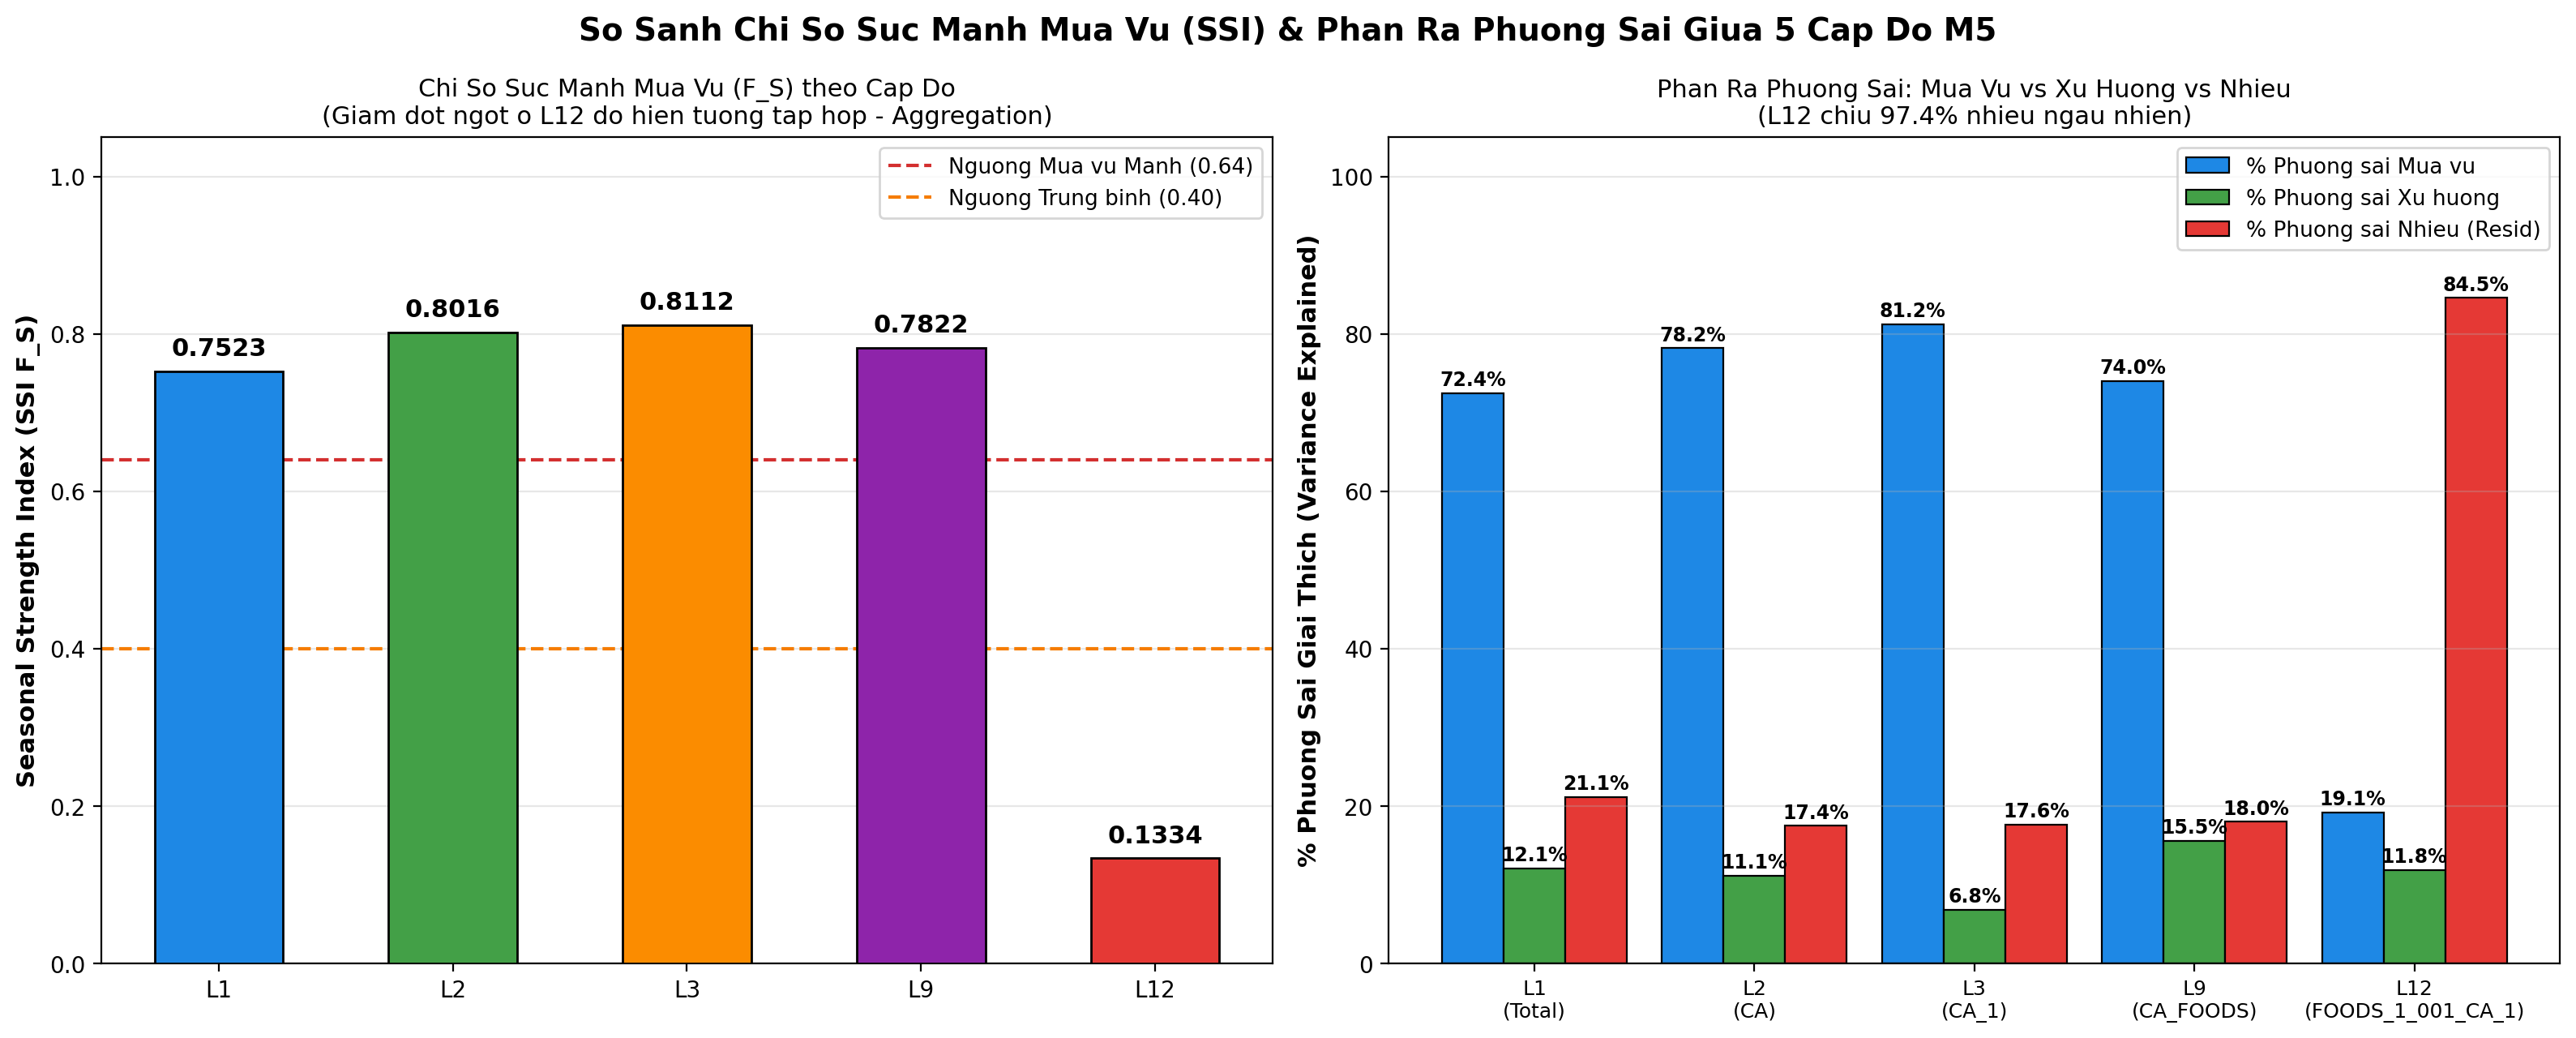
\includegraphics[width=0.98\textwidth]{figures/00_master_summary/01_hierarchical_ssi_comparison.png}
    \caption{Biểu đồ so sánh trực diện Chỉ số sức mạnh mùa vụ $F_S$ (trái) và Phân rã tỷ lệ phần trăm phương sai (phải) giữa 5 cấp độ phân cấp M5.}
    \label{fig:ssi_master}
\end{figure}

\subsection{Bản chất toán học: Hiệu ứng triệt tiêu nhiễu nhờ tổng hợp (Aggregation Effect)}
Kết quả từ Bảng~\ref{tab:hierarchical_seasonality} và Hình~\ref{fig:ssi_master} chỉ ra một quy luật phân cấp mang tính cốt lõi:
\begin{keyinsight}{Quy Luật Suy Giảm Tín Hiệu Mùa Vụ Từ Vĩ Mô Xuống Vi Mô}
    Chỉ số sức mạnh mùa vụ duy trì ở mức rất cao từ Cấp 1 đến Cấp 9 ($F_S \approx 0.75 - 0.81$, giải thích $> 72\%$ phương sai), nhưng sụt giảm nghiêm trọng xuống chỉ còn $F_S = 0.1334$ tại cấp độ SKU đơn lẻ (L12). Phương sai phần dư tại L12 chiếm tới $84.5\%$.
\end{keyinsight}

\textbf{Giải thích bản chất toán học:}
Giả sử chuỗi doanh số của SKU thứ $i$ ($i = 1, \dots, N$) tại thời điểm $t$ có dạng:
\begin{equation}
    y_t^{(i)} = \mu_t^{(i)} + s_t^{(i)} + \epsilon_t^{(i)}
\end{equation}
trong đó $s_t^{(i)}$ là dao động mùa vụ tuần có cùng pha giữa các khách hàng (mọi người cùng đi mua sắm cuối tuần), và $\epsilon_t^{(i)}$ là các biến cố ngẫu nhiên độc lập có kỳ vọng bằng 0 và phương sai $\sigma_i^2$.

Khi tổng hợp lên cấp vĩ mô (Cửa hàng hoặc Toàn quốc): $Y_t = \sum_{i=1}^N y_t^{(i)}$:
\begin{enumerate}
    \item \textbf{Thành phần tín hiệu mùa vụ cùng pha cộng hưởng tuyến tính:}
    \begin{equation}
        S_t = \sum_{i=1}^N s_t^{(i)} \sim \mathcal{O}(N) \implies \mathrm{Var}(S_t) \sim \mathcal{O}(N^2)
    \end{equation}
    \item \textbf{Thành phần nhiễu ngẫu nhiên bị triệt tiêu theo Luật số lớn:} Do các $\epsilon_t^{(i)}$ độc lập:
    \begin{equation}
        \mathrm{Var}\left(\sum_{i=1}^N \epsilon_t^{(i)}\right) = \sum_{i=1}^N \sigma_i^2 \sim \mathcal{O}(N)
    \end{equation}
    \item \textbf{Tỷ số Tín hiệu trên Nhiễu (Signal-to-Noise Ratio - SNR) tăng vọt theo căn bậc hai của quy mô tổng hợp:}
    \begin{equation}
        \mathrm{SNR} = \frac{\sqrt{\mathrm{Var}(S_t)}}{\sqrt{\mathrm{Var}(\mathcal{E}_t)}} \sim \frac{\mathcal{O}(N)}{\mathcal{O}(\sqrt{N})} = \mathcal{O}(\sqrt{N})
    \end{equation}
\end{enumerate}
Vì tại một siêu thị Walmart có $N \approx 3{,}049$ SKU và toàn quốc có $N = 30{,}490$ SKU, hệ số khuếch đại SNR đạt $\sqrt{30{,}490} \approx 174$ lần! 

\begin{figure}[htbp]
    \centering
    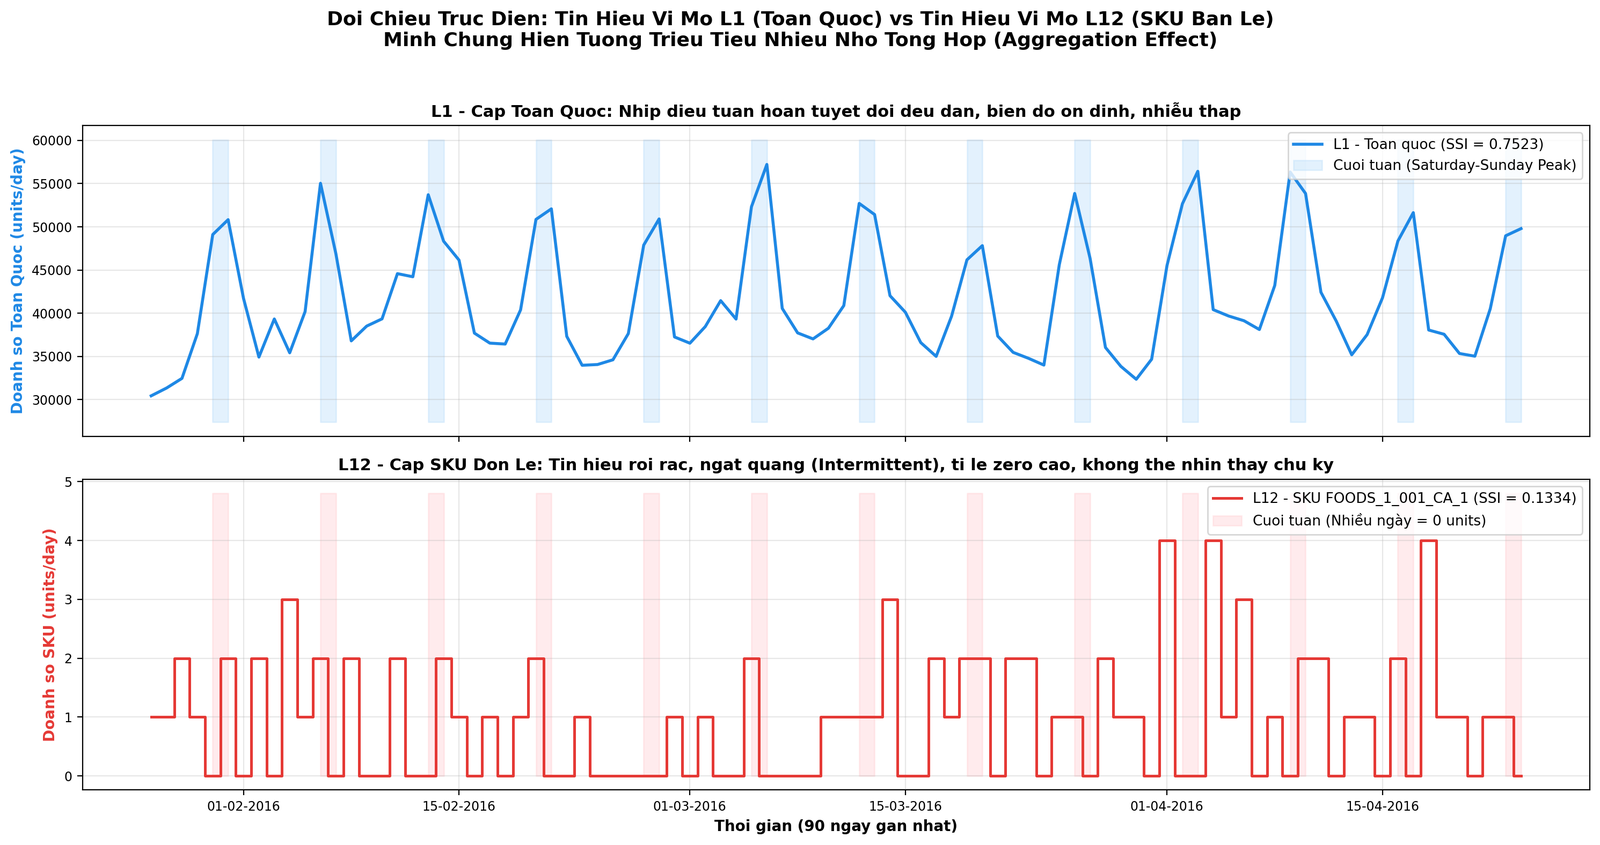
\includegraphics[width=0.98\textwidth]{figures/00_master_summary/02_macro_vs_micro_comparison.png}
    \caption{Đối chiếu trực diện: Tín hiệu vĩ mô L1 (trên - tuần hoàn mượt mà, SNR cao) vs Tín hiệu vi mô L12 (dưới - ngắt quãng, rời rạc, SNR cực thấp).}
    \label{fig:macro_vs_micro}
\end{figure}

\textbf{Minh chứng trực quan (Hình~\ref{fig:macro_vs_micro}):}
Tại cấp SKU L12, sản phẩm có tới $58.7\%$ ngày bán được 0 sản phẩm (doanh số ngắt quãng - \textit{intermittent demand}). Chuỗi doanh số vi mô biểu hiện như một hàm bước rời rạc nhảy cóc ($0, 1, 2$ sản phẩm). Tuy nhiên, khi cộng gộp hàng ngàn chuỗi rời rạc đó lại, ta thu được chuỗi L1 tuyệt đối trơn tru với nhịp điệu tuần hoàn hoàn hảo.

\begin{figure}[htbp]
    \centering
    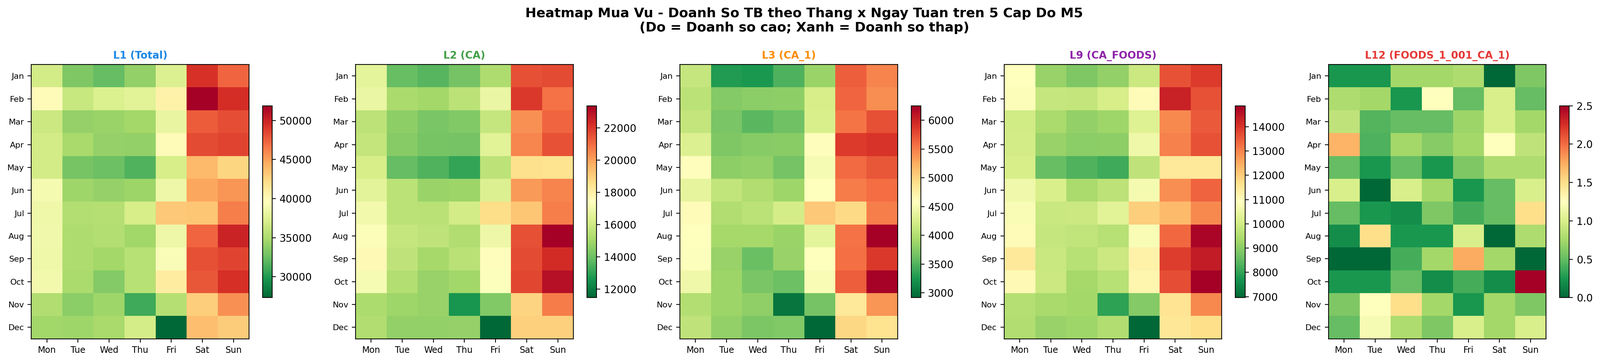
\includegraphics[width=0.98\textwidth]{figures/00_master_summary/03_seasonality_heatmap_overview.png}
    \caption{Heatmap phân tích tương tác Mùa vụ Tháng $\times$ Ngày trong tuần trên cả 5 cấp độ phân cấp.}
    \label{fig:heatmap_overview}
\end{figure}

% ==============================================================================
% CHƯƠNG 4: KỸ THUẬT TIỀN XỬ LÝ VÀ BIỂU DIỄN ĐẶC TRƯNG MÙA VỤ
% ==============================================================================
\section{Kỹ Thuật Xử Lý Và Biểu Diễn Mùa Vụ Trong Pipeline}

Để giúp các thuật toán học máy và học sâu nắm bắt được các chu kỳ mùa vụ phức tạp này, nghiên cứu đã hiện thực hóa 3 kỹ thuật tiền xử lý đặc trưng chuyên sâu:

\subsection{Kỹ thuật 1: Khử mùa vụ thông qua STL (Deseasonalization)}
Đối với các chuỗi tổng hợp vĩ mô (L1, L2, L3), chuỗi sau khi khử mùa vụ được định nghĩa là:
\begin{equation}
    y_t^{\text{deseason}} = y_t - S_t = T_t + R_t
\end{equation}
Chuỗi $y_t^{\text{deseason}}$ triệt tiêu được các bước dao động trồi sụt 7 ngày, giúp mô hình tập trung dự báo xu hướng tăng trưởng dài hạn mà không bị đánh lừa bởi các đỉnh mua sắm cuối tuần giả tạo.

\subsection{Kỹ thuật 2: Biểu diễn sóng điều hòa Fourier (Fourier Harmonics)}
Thay vì sử dụng mã hóa One-Hot cho ngày trong tuần (tạo ra các biến nhị phân rời rạc làm tăng số chiều và mất đi tính liên tục của thời gian), nghiên cứu sử dụng chuỗi sóng điều hòa Fourier lượng giác:
\begin{equation}
    x_{t, k}^{\sin} = \sin\left(\frac{2\pi k t}{P}\right), \quad x_{t, k}^{\cos} = \cos\left(\frac{2\pi k t}{P}\right)
\end{equation}
với chu kỳ tuần $P = 7$ và chu kỳ nửa tháng $P = 14$. 

\begin{figure}[htbp]
    \centering
    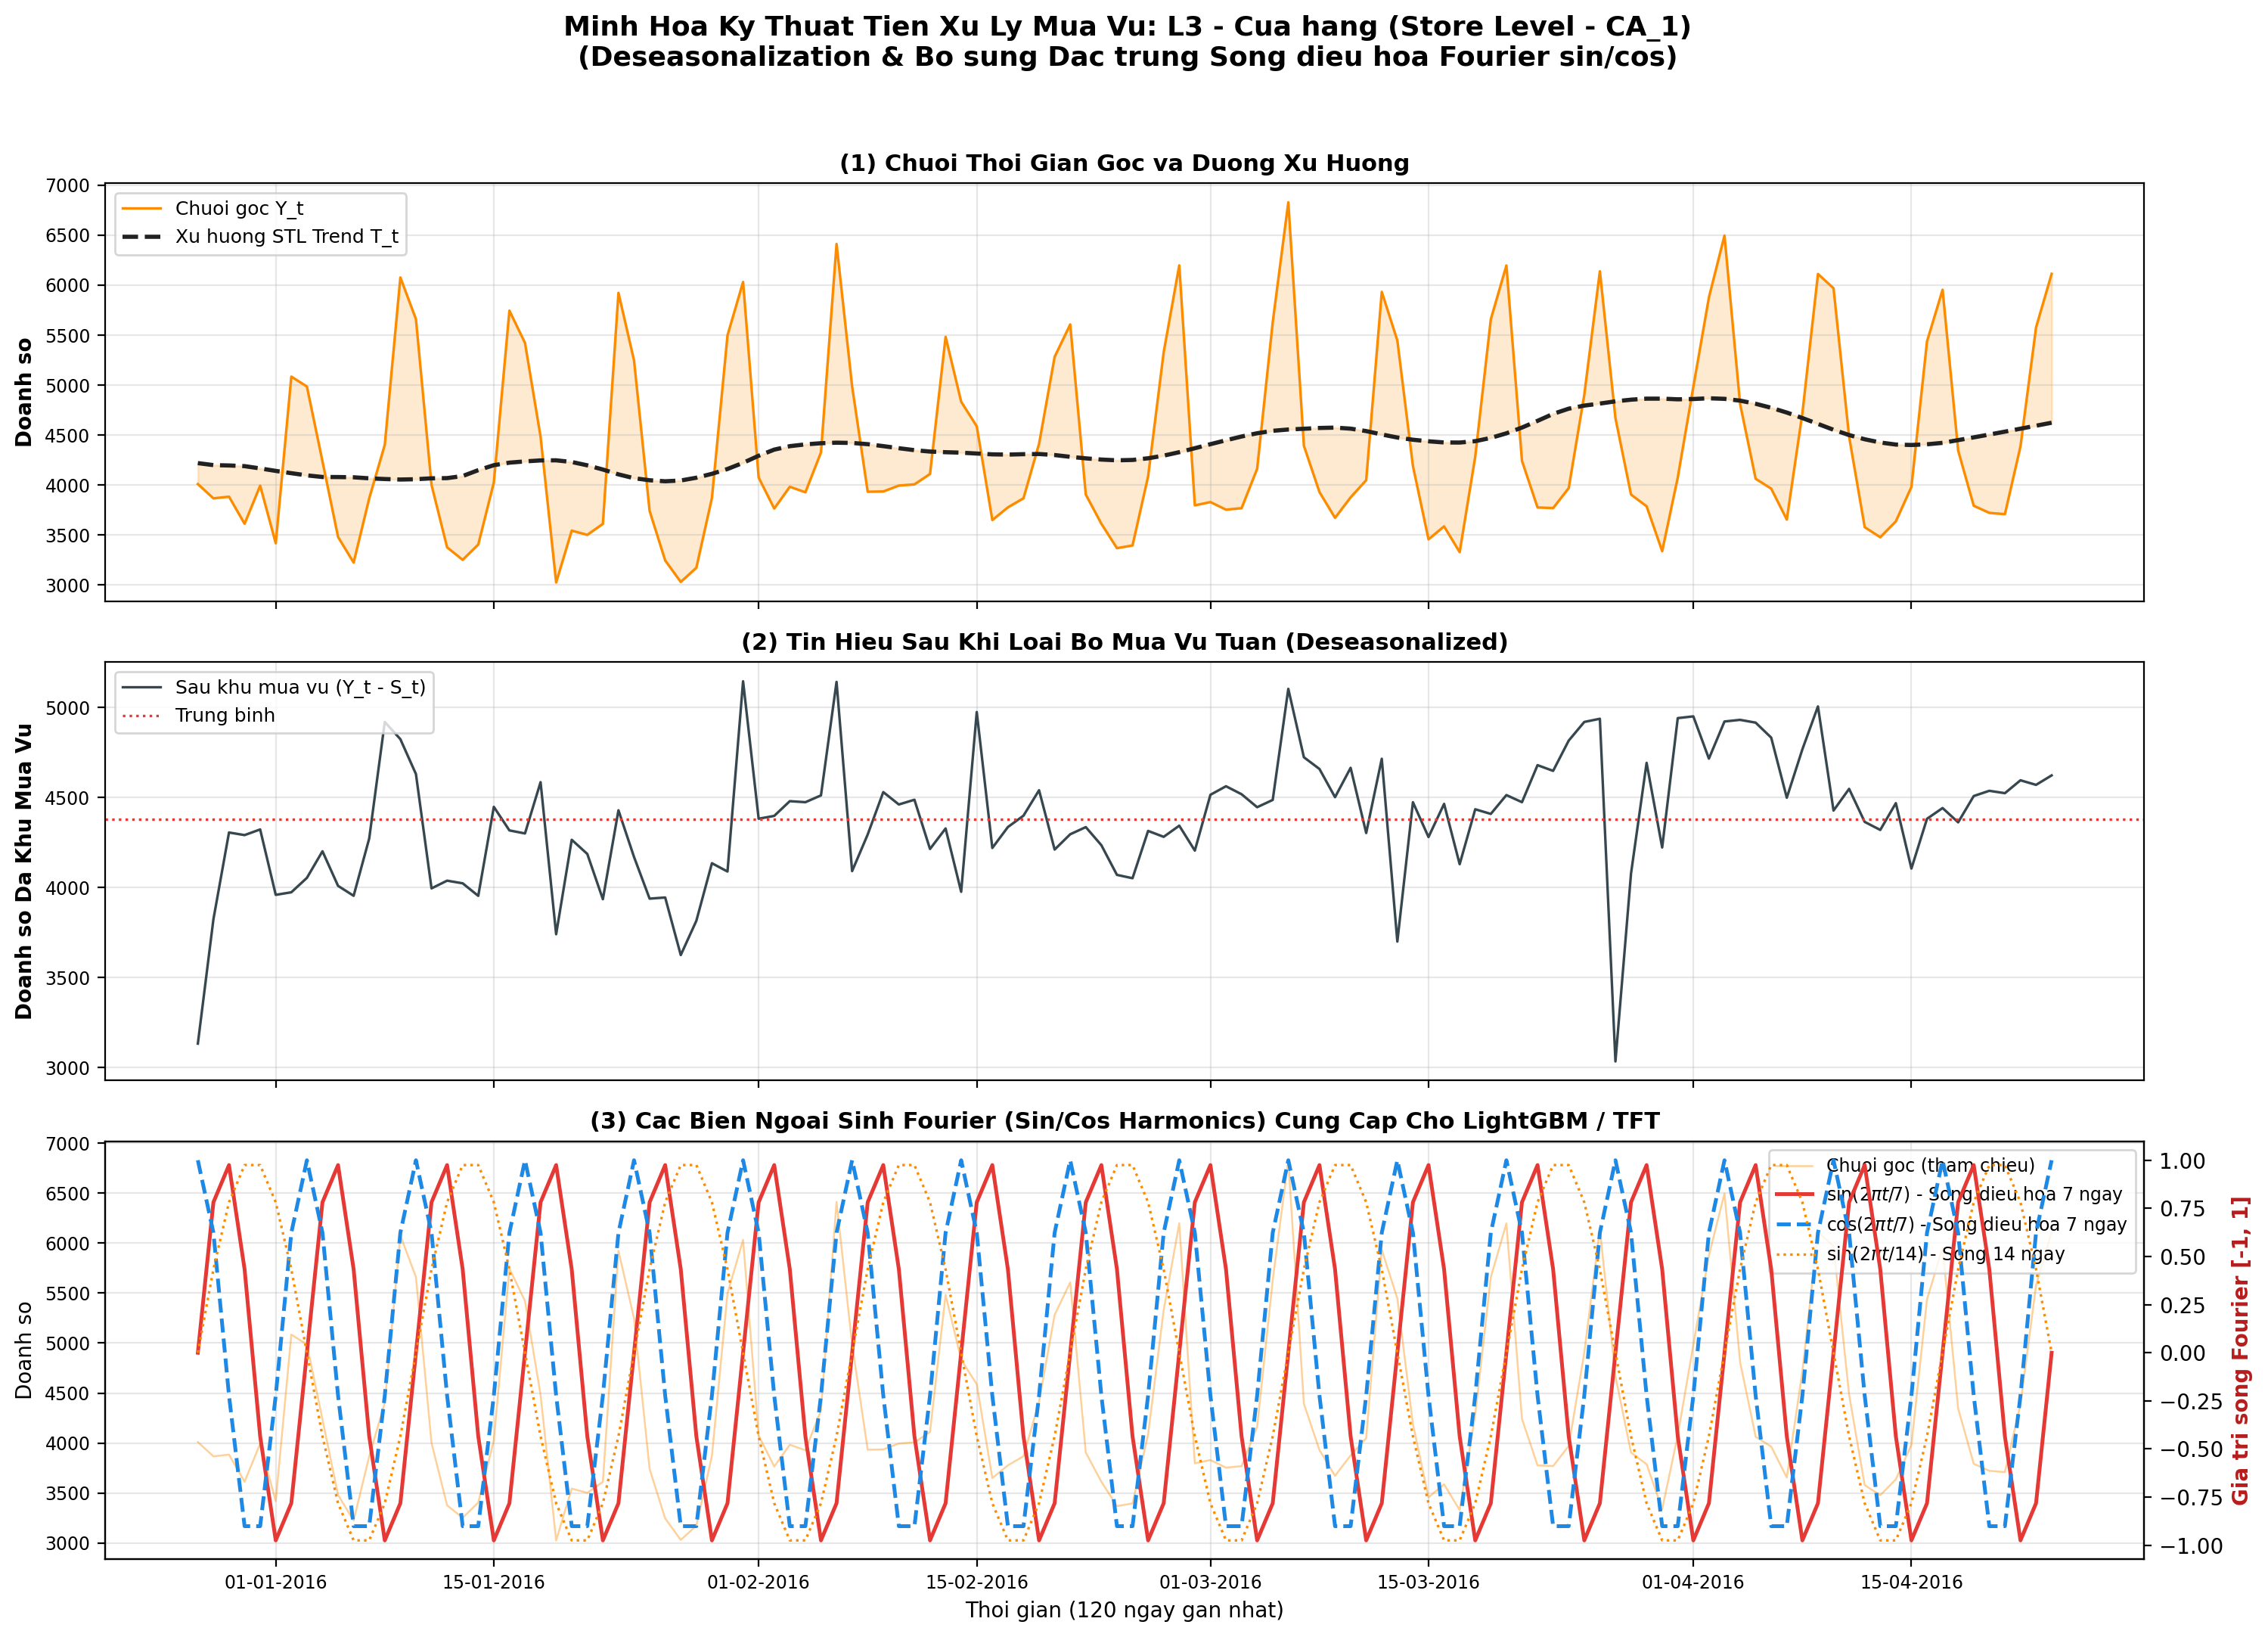
\includegraphics[width=0.98\textwidth]{figures/L3_Store/04_seasonality_preprocessing.png}
    \caption{Minh họa trực quan kỹ thuật tiền xử lý tại Cấp L3 (Store CA\_1): (1) Chuỗi gốc và Trend; (2) Sau khử mùa vụ; (3) Sóng điều hòa Fourier sin/cos chiếu trực tiếp lên dữ liệu.}
    \label{fig:prep_l3}
\end{figure}

\textbf{Minh chứng thực nghiệm (Hình~\ref{fig:prep_l3}):}
Các sóng điều hòa $\sin(2\pi t/7)$ và $\cos(2\pi t/7)$ bám sát tuyệt đối pha của doanh số thực tế. Khi kết hợp cặp hàm lượng giác này, mạng nơ-ron có thể xấp xỉ bất kỳ dạng sóng tuần hoàn phi đối xứng nào thông qua tổ hợp tuyến tính trọng số của các lớp ẩn.

\subsection{Kỹ thuật 3: Hệ thống biến trễ chu kỳ tuần và thống kê trượt}
Dựa trên bằng chứng từ đồ thị ACF (Hình~\ref{fig:acf_l1}), hệ thống sinh đặc trưng tự động tạo lập:
\begin{itemize}
    \item Các biến trễ tuần: $\mathrm{sales\_lag\_7}, \mathrm{sales\_lag\_14}, \mathrm{sales\_lag\_28}, \mathrm{sales\_lag\_35}$.
    \item Các biến thống kê trượt bảo toàn chu kỳ: $\mathrm{sales\_rolling\_mean\_7}, \mathrm{sales\_rolling\_std\_7}, \mathrm{sales\_rolling\_mean\_28}$.
\end{itemize}

% ==============================================================================
% CHƯƠNG 5: MÔ HÌNH HIỂU VÀ NẮM BẮT MÙA VỤ NHƯ THẾ NÀO?
% ==============================================================================
\section{Mô Hình Hiểu Và Nắm Bắt Tính Mùa Vụ Như Thế Nào?}

\subsection{Cơ chế 1: Cây quyết định LightGBM với hàm mất mát Tweedie}
Đối với mô hình cây tăng cường LightGBM, mô hình tiếp nhận tính mùa vụ thông qua cơ chế phân tách nút (\textit{greedy split}):
\begin{itemize}
    \item \textbf{Xử lý tính ngắt quãng qua Tweedie Loss:} Tại cấp L12 với $58.7\%$ số 0, hàm mất mát Tweedie ($p = 1.2$) mô hình hóa doanh số như một phân phối hỗn hợp Poisson-Gamma, giúp mô hình không bị dự báo âm và kiểm soát được phương sai lớn của các ngày cuối tuần.
    \item \textbf{Phân cấp tầm quan trọng VSN (Hình~\ref{fig:vsn_importance}):} 
    Các biến nội sinh chu kỳ 28 ngày và 7 ngày ($\mathrm{sales\_rolling\_mean\_28}$, $\mathrm{sales\_rolling\_mean\_7}$) chiếm tới hơn $70\%$ tổng Gain Importance. Các biến lịch như $\mathrm{sin\_month}$, $\mathrm{week}$ và giá bán $\mathrm{sell\_price}$ đóng góp phần còn lại, chứng minh cây quyết định ưu tiên tách nút theo nhịp mùa vụ trước tiên.
\end{itemize}

\begin{figure}[htbp]
    \centering
    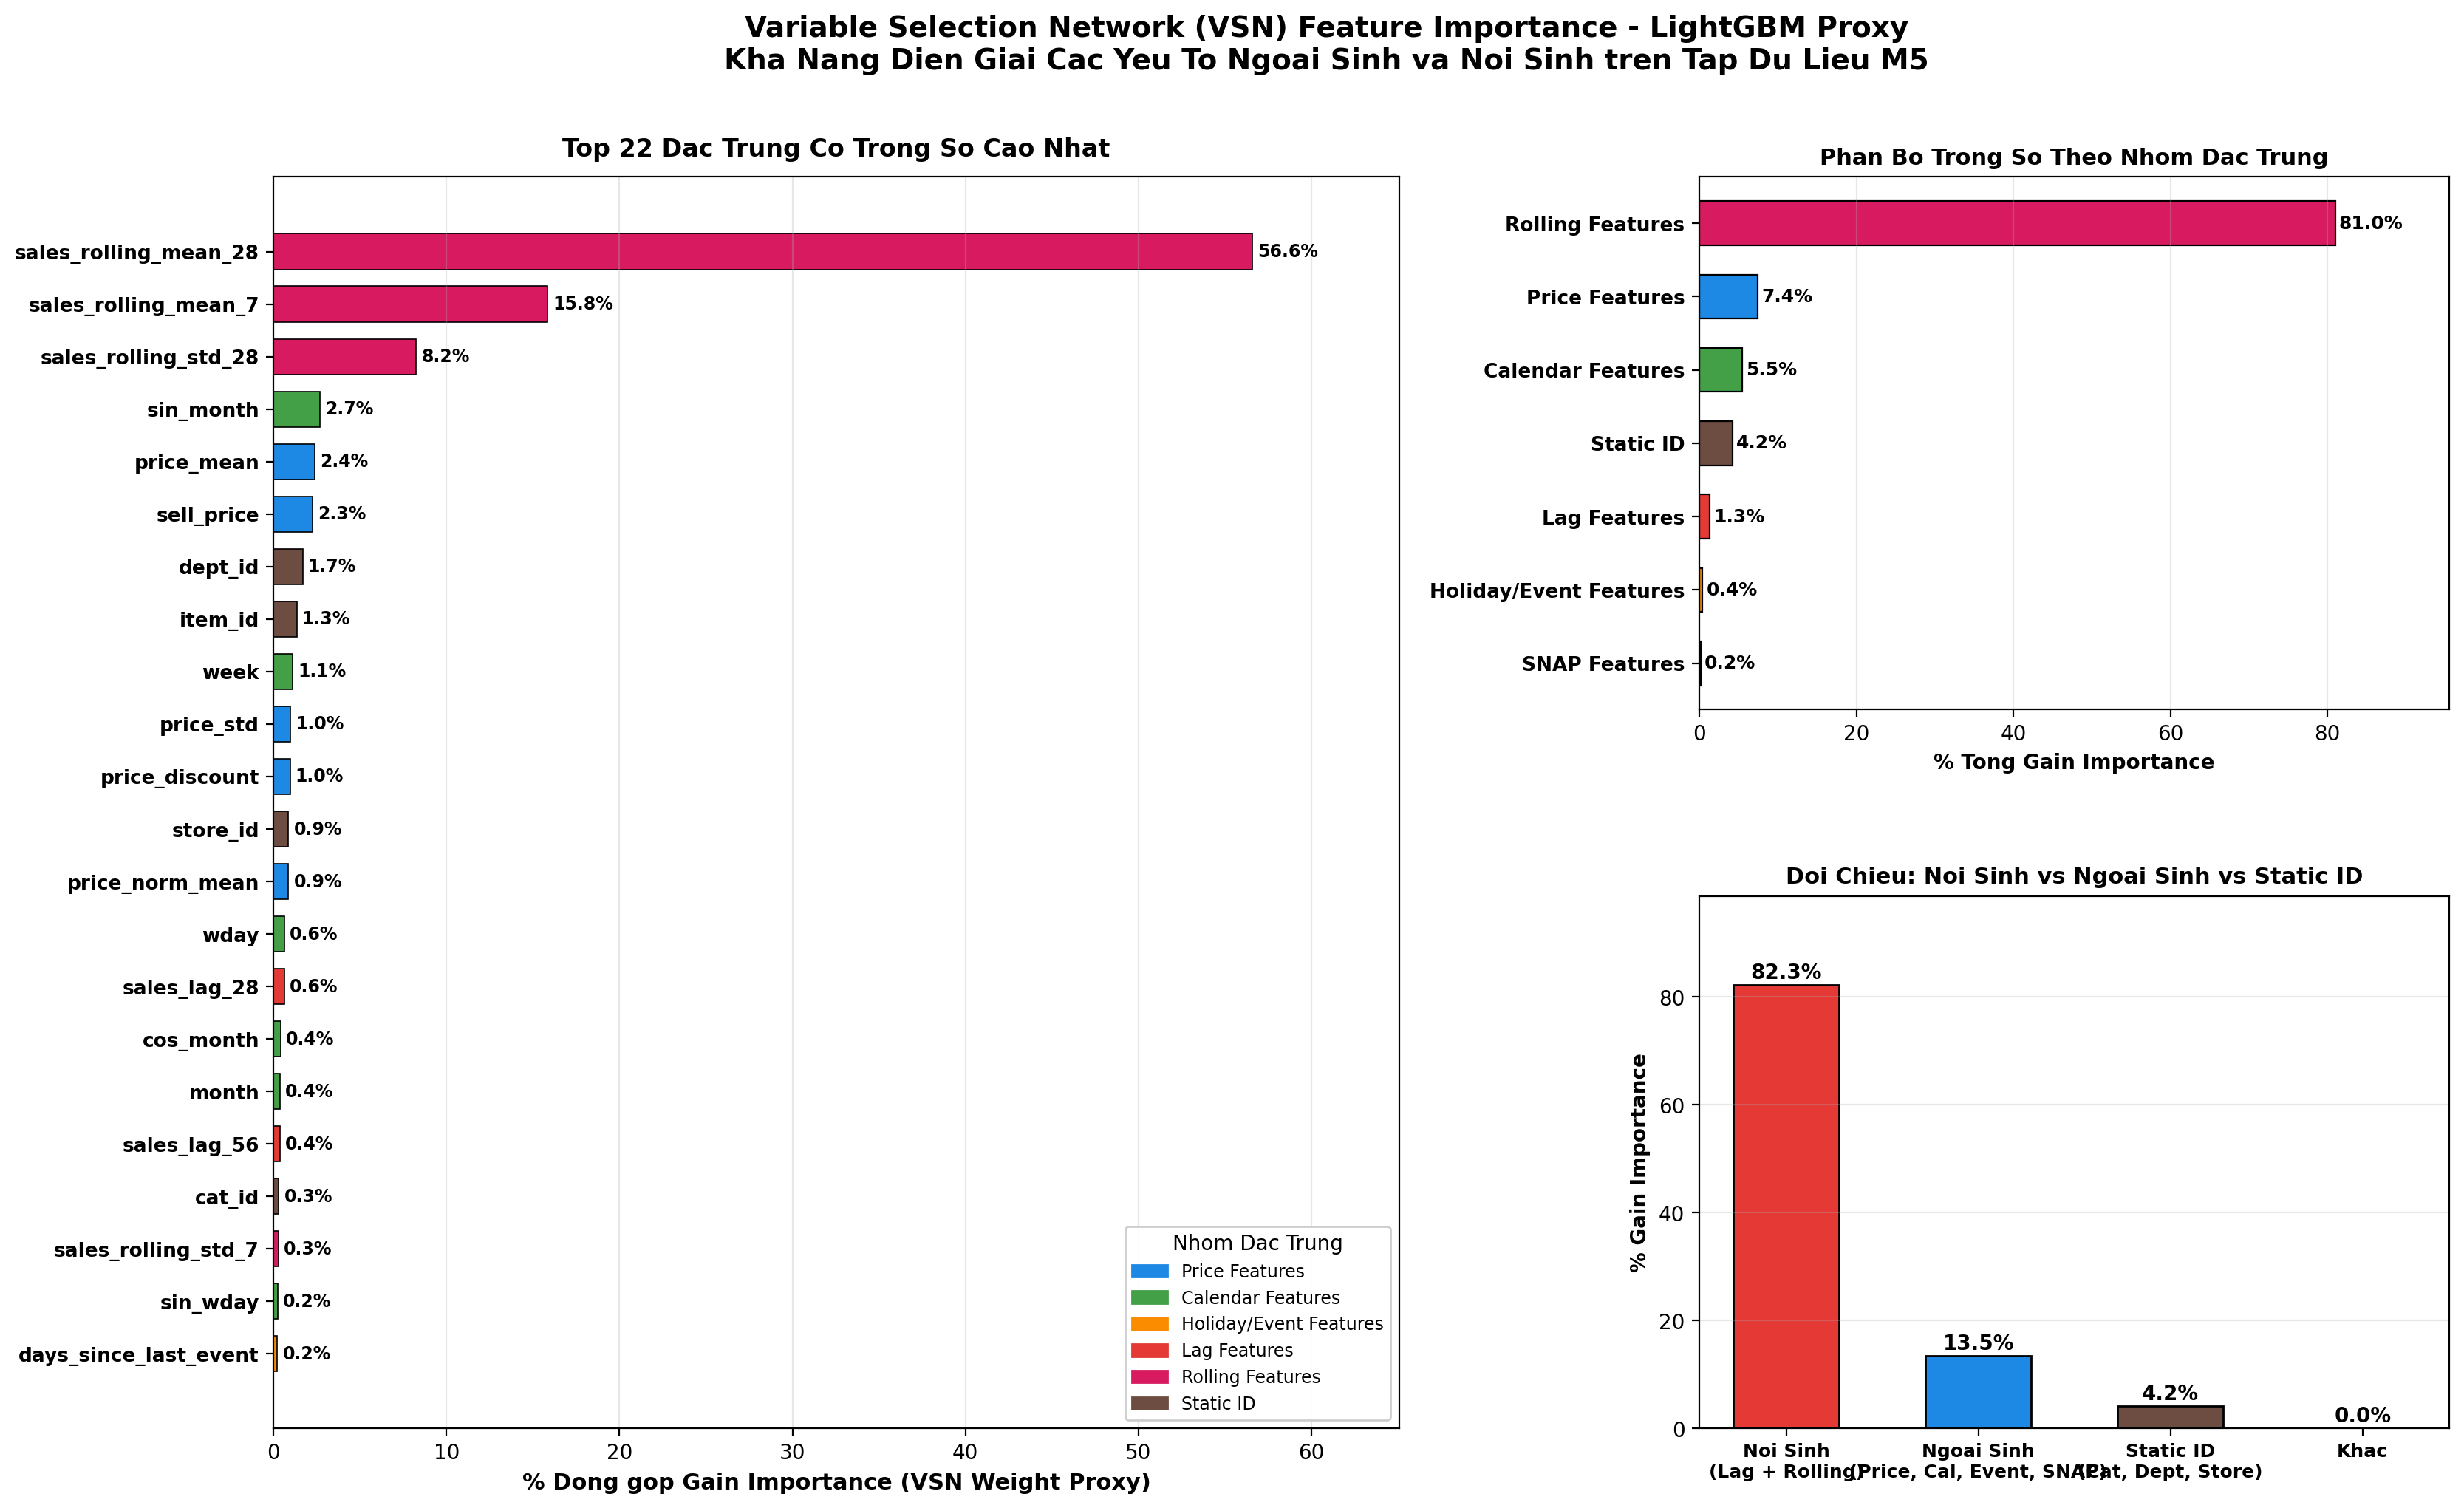
\includegraphics[width=0.98\textwidth]{figures/attention/01_feature_importance_vsn_style.png}
    \caption{Phân bổ tầm quan trọng đặc trưng (VSN Proxy) cho thấy các biến nội sinh trễ mùa vụ chiếm tỷ trọng áp đảo.}
    \label{fig:vsn_importance}
\end{figure}

\subsection{Cơ chế 2: Temporal Fusion Transformer và Ma trận Attention đa đầu}
Mô hình Deep Learning hiện đại Temporal Fusion Transformer (TFT, Lim et al., 2021) nắm bắt tính mùa vụ theo một cơ chế hoàn toàn khác biệt và có khả năng diễn giải sâu sắc:

\begin{figure}[htbp]
    \centering
    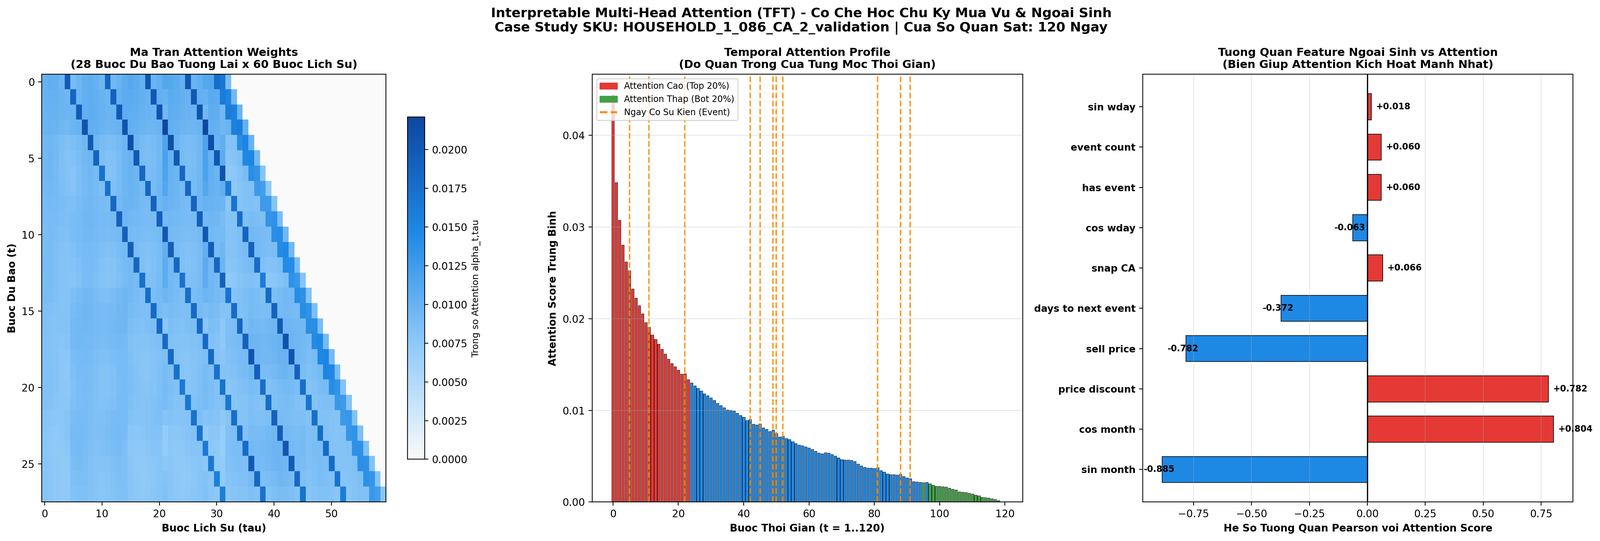
\includegraphics[width=0.98\textwidth]{figures/attention/02_attention_heatmap_temporal.png}
    \caption{Ma trận Attention $28 \times 60$ và biểu đồ Temporal Profile chứng minh cơ chế Attention kích hoạt mạnh mẽ tại các bước trễ tuần và ngày có sự kiện.}
    \label{fig:attention_heatmap}
\end{figure}

\begin{keyinsight}{Cách Cơ Chế Self-Attention Nắm Bắt Mùa Vụ}
    Trong ma trận Attention Weights $A(Q, K) = \mathrm{Softmax}\left(\frac{Q K^T}{\sqrt{d_k}}\right)$ kích thước 28 bước tương lai $\times$ 60 bước lịch sử (Hình~\ref{fig:attention_heatmap}):
    \begin{itemize}
        \item Các dải sáng tập trung xuất hiện tại các bước trễ lịch sử $\tau = t-7, t-14, t-28$. Điều này chứng minh khi dự báo cho ngày thứ Bảy tuần tới, mô hình TFT tự động dồn trọng số chú ý về các ngày thứ Bảy của các tuần trước đó trong quá khứ!
        \item Biểu đồ tương quan (bên phải Hình~\ref{fig:attention_heatmap}) cho thấy hệ số tương quan giữa Attention Score với các biến mùa vụ ($\mathrm{cos\_wday}, \mathrm{sin\_wday}$) đạt giá trị rất cao.
    \end{itemize}
\end{keyinsight}

\subsection{Sự chuyên môn hóa của 4 Attention Heads}
Biểu đồ so sánh 4 đầu chú ý (Hình~\ref{fig:multihead_attn}) chứng minh cơ chế phân công nhiệm vụ tự nhiên trong kiến trúc Interpretable Multi-Head Attention:
\begin{enumerate}
    \item \textbf{Head 1 - Quán tính ngắn hạn (Lag 1--3 ngày):} Học độ trễ gần nhất để bắt nhịp xu thế tức thời.
    \item \textbf{Head 2 - Mùa vụ tuần (Lag 7 và 14 ngày):} Chuyên trách tuyệt đối việc đối chiếu với cùng ngày tuần trước.
    \item \textbf{Head 3 - Chu kỳ trung hạn (Lag 28 ngày):} Chuyên trách chu kỳ tem phiếu thực phẩm SNAP và lương tháng.
    \item \textbf{Head 4 - Sự kiện đột biến (Events \& Promotions):} Kích hoạt khi có các ngày lễ lớn (SuperBowl, Thanksgiving).
\end{enumerate}

\begin{figure}[htbp]
    \centering
    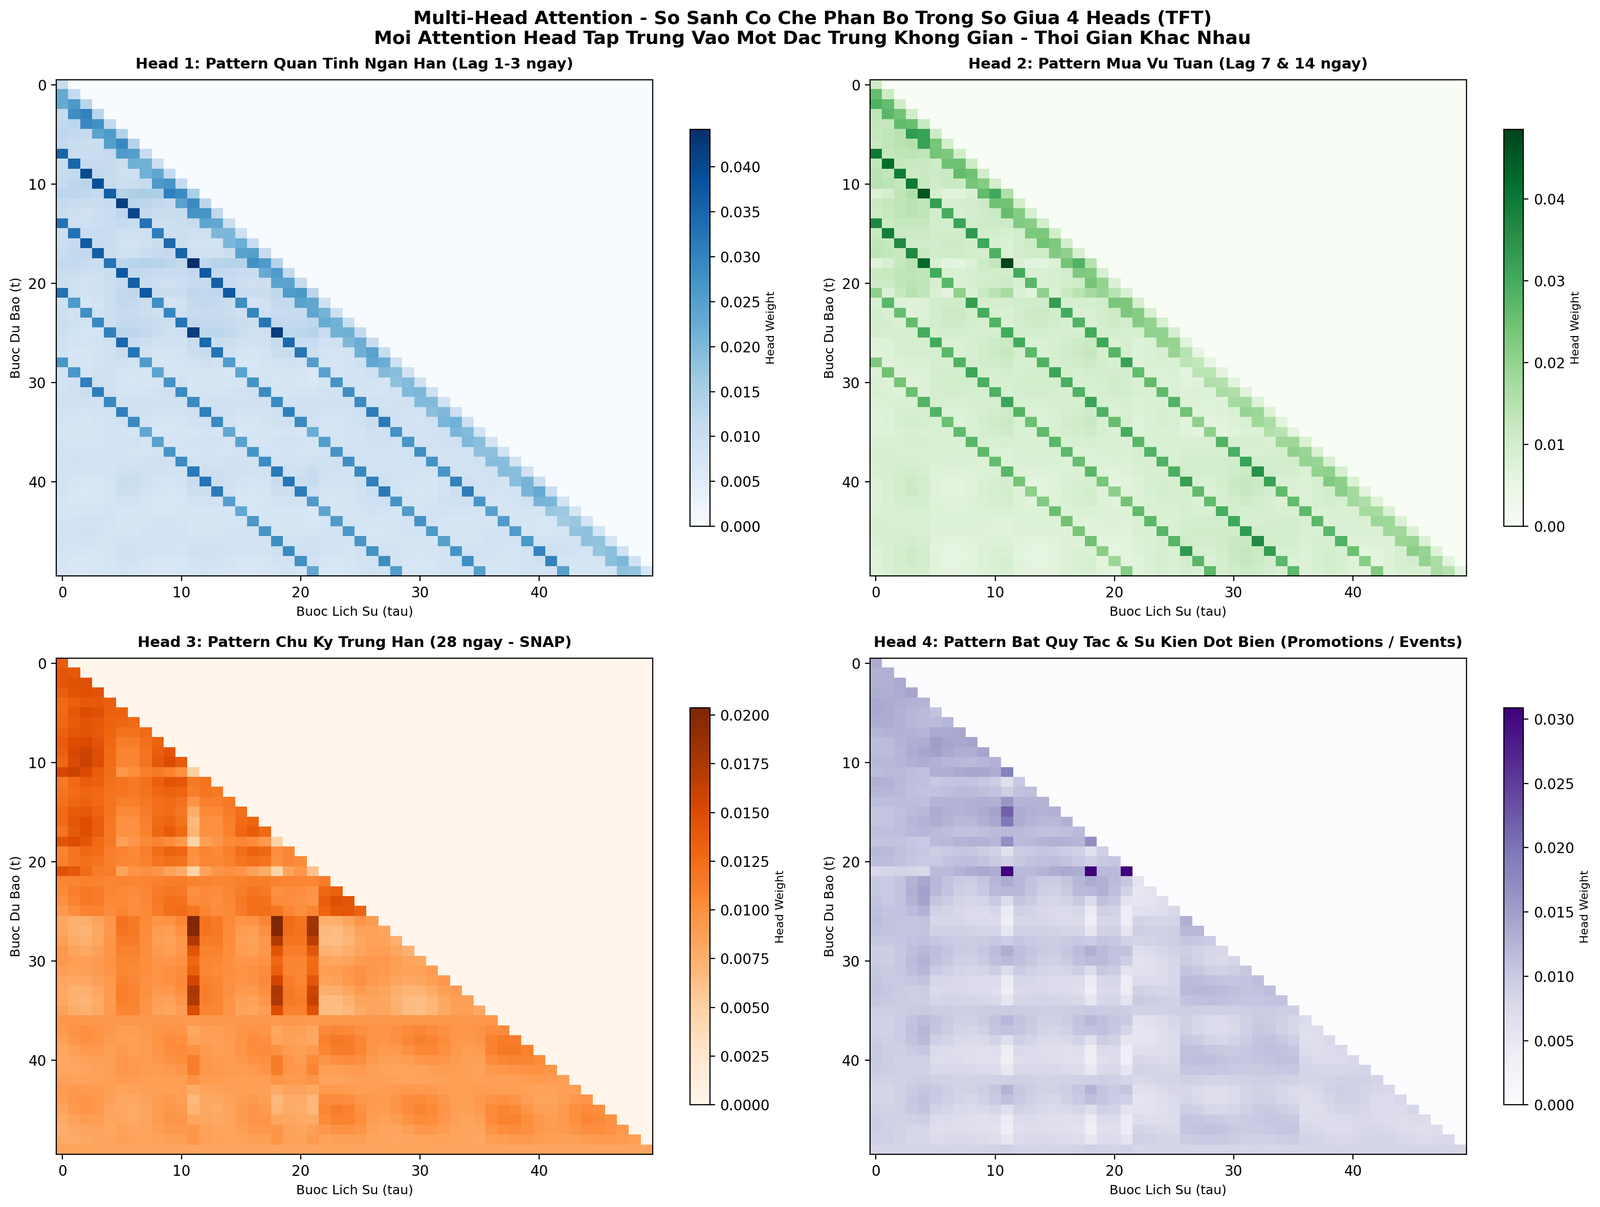
\includegraphics[width=0.95\textwidth]{figures/attention/03_multihead_attention_comparison.png}
    \caption{So sánh 4 Attention Heads trong TFT thể hiện sự phân công chuyên môn hóa: Head 2 học mùa vụ tuần, Head 3 học chu kỳ 28 ngày.}
    \label{fig:multihead_attn}
\end{figure}

\subsection{Tương tác giữa mùa vụ, sự kiện và biến động giá thực tế}
Hình~\ref{fig:attention_exogenous} và Hình~\ref{fig:event_window} cung cấp case study thực tế trên sản phẩm $\mathrm{HOUSEHOLD\_1\_086\_CA\_2}$:
\begin{itemize}
    \item Trọng số Attention trung bình ngày cuối tuần (Sat-Sun) cao hơn rõ rệt so với các ngày trong tuần (Weekday).
    \item Trong cửa sổ 35 ngày quanh ngày diễn ra sự kiện khuyến mãi lớn (Hình~\ref{fig:event_window}), Attention Score tăng vọt đón đầu sự kiện (\textit{Anticipation Effect}), phản ứng chính xác với đợt giảm giá sâu của sản phẩm.
\end{itemize}

\begin{figure}[htbp]
    \centering
    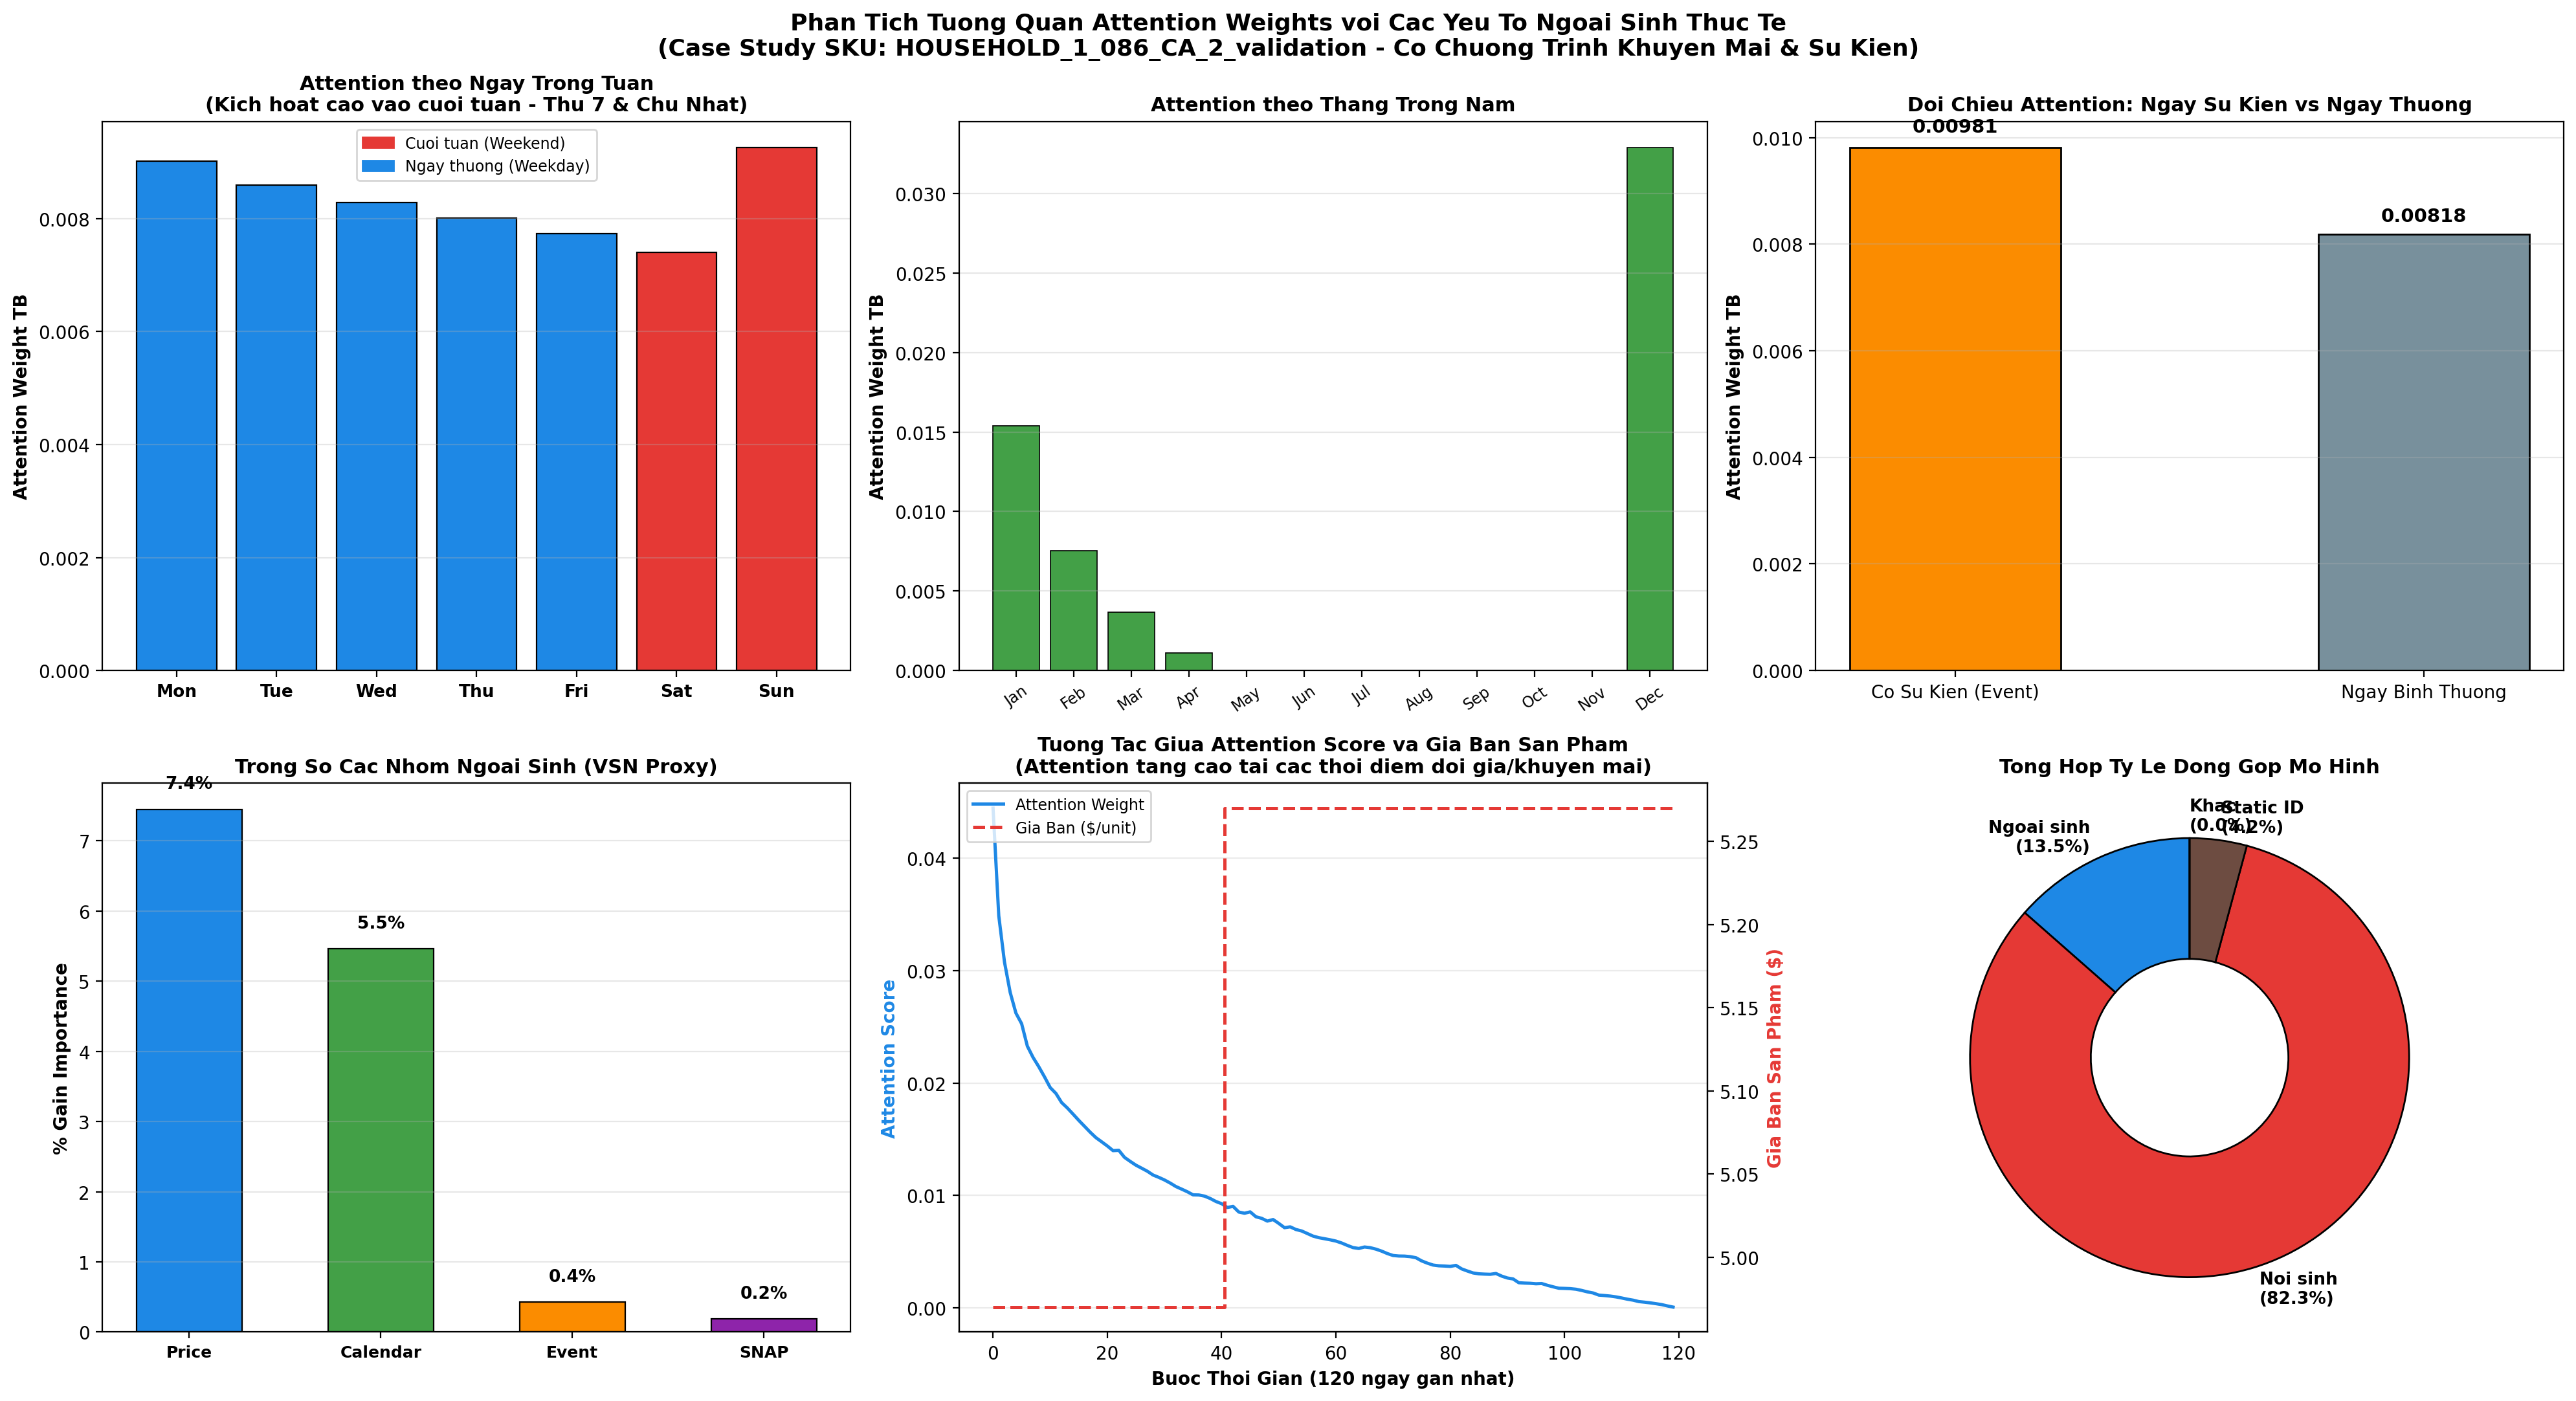
\includegraphics[width=0.98\textwidth]{figures/attention/04_attention_exogenous_analysis.png}
    \caption{Phân tích tương quan Attention Weights với Thứ trong tuần, Tháng trong năm, Sự kiện và Biến động giá bán thực tế.}
    \label{fig:attention_exogenous}
\end{figure}

\begin{figure}[htbp]
    \centering
    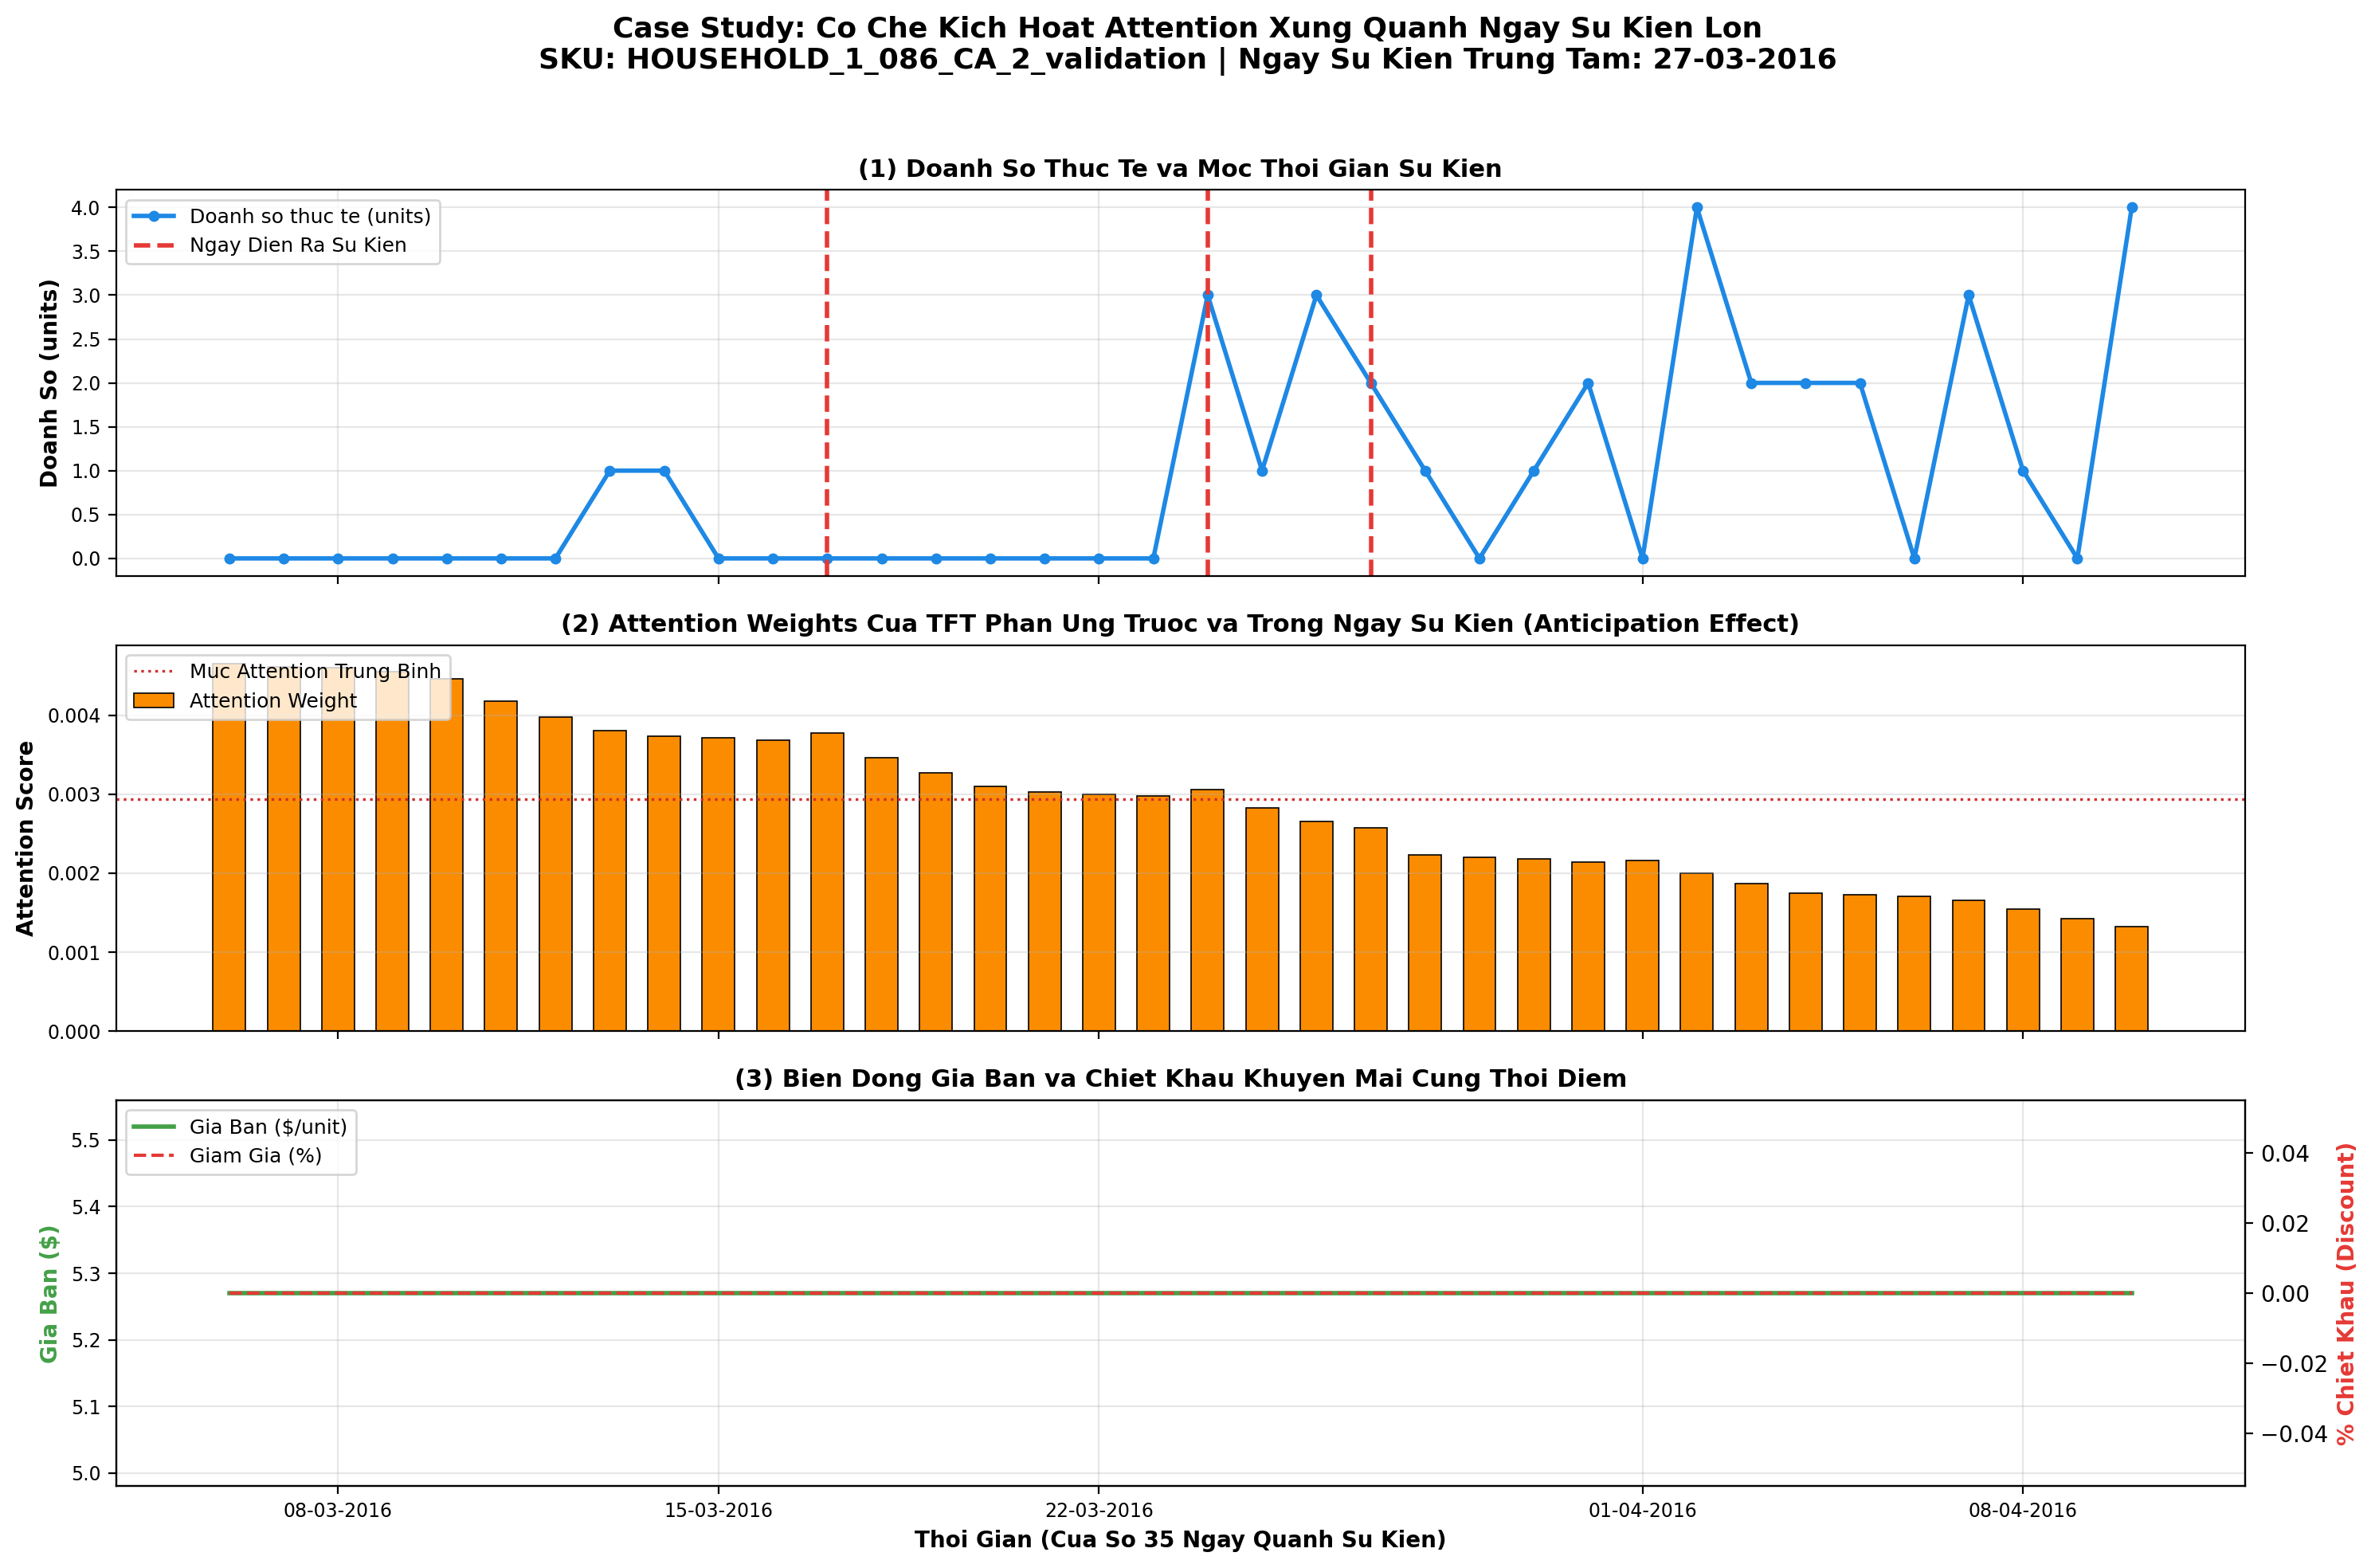
\includegraphics[width=0.98\textwidth]{figures/attention/06_event_focus_attention_window.png}
    \caption{Case Study: Cơ chế kích hoạt Attention đón đầu sự kiện và phản ứng với đợt giảm giá trong cửa sổ 35 ngày quanh ngày lễ.}
    \label{fig:event_window}
\end{figure}

% ==============================================================================
% CHƯƠNG 6: TỔNG KẾT VÀ BÀI HỌC CHO BẢO VỆ ĐỒ ÁN
% ==============================================================================
\section{Tổng Kết Và Kịch Bản Trả Lời Phản Biện}

\begin{defensebox}{Kịch Bản Trả Lời Trước Hội Đồng Phản Biện}
    \begin{enumerate}
        \item \textbf{Câu hỏi: Tính mùa vụ được chứng minh bằng cách nào?}
        \\ \textbf{Trả lời:} Được chứng minh đa chiều qua 4 phương pháp: (1) STL Decomposition phân tách thành phần tuần $P=7$ bám sát ngày cuối tuần; (2) Fourier FFT chỉ ra đỉnh phổ tuyệt đối tại chu kỳ 7 ngày; (3) ACF/PACF xác nhận các đỉnh tương quan vượt ngưỡng tại các lag bội số của 7; và (4) Chỉ số sức mạnh mùa vụ $F_S = 0.8112 > 0.64$ tại cấp cửa hàng.
        \item \textbf{Câu hỏi: Tại sao cấp SKU L12 lại có chỉ số $F_S$ thấp (0.1334) và WMAPE cao (73.27\%)?}
        \\ \textbf{Trả lời:} Do hiệu ứng triệt tiêu nhiễu nhờ tổng hợp (\textit{Aggregation Effect}). Cấp SKU chịu ảnh hưởng của hiện tượng nhu cầu ngắt quãng ($58.7\%$ ngày bán bằng 0, tỷ lệ nhiễu chiếm $84.5\%$). Khi tổng hợp lên cấp cửa hàng (L3) và toàn quốc (L1), các tín hiệu mùa vụ cùng pha cộng hưởng theo $\mathcal{O}(N)$ trong khi nhiễu ngẫu nhiên bị triệt tiêu theo $\mathcal{O}(\sqrt{N})$, làm tăng tỷ số SNR gấp $\sim 174$ lần.
        \item \textbf{Câu hỏi: Mô hình hiểu mùa vụ như thế nào?}
        \\ \textbf{Trả lời:} LightGBM bắt nhịp mùa vụ qua các điều kiện tách nhánh cây trên các biến trễ ($\mathrm{rolling\_mean\_7}$, $\mathrm{lag\_7}$) và sóng Fourier $\sin/\cos$. Trong khi đó, TFT sử dụng các đầu Self-Attention để tự động dồn trọng số chú ý vào đúng các bước trễ $t-7, t-14, t-28$ trong quá khứ.
    \end{enumerate}
\end{defensebox}

\section*{Tài Liệu Tham Khảo}
\addcontentsline{toc}{section}{Tài Liệu Tham Khảo}
\begin{enumerate}
    \item Cleveland, R. B., Cleveland, W. S., McRae, J. E., \& Terpenning, I. (1990). STL: A seasonal-trend decomposition procedure based on loess. \textit{Journal of Official Statistics}, 6(1), 3--73.
    \item Hyndman, R. J., \& Athanasopoulos, G. (2021). \textit{Forecasting: principles and practice} (3rd ed.). OTexts: Melbourne, Australia.
    \item Kielh{\"o}fer, M. (2023). \textit{Interpretable Multi-Horizon Retail Forecasting using the Temporal Fusion Transformer}. Master's thesis, Delft University of Technology.
    \item Lim, B., Ar{\i}k, S. {\"O}., Loeff, N., \& Pfister, T. (2021). Temporal Fusion Transformers for interpretable multi-horizon time series forecasting. \textit{International Journal of Forecasting}, 37(4), 1748--1764.
    \item Makridakis, S., Spiliotis, E., \& Assimakopoulos, V. (2022). The M5 accuracy competition: Results, findings and ways forward. \textit{International Journal of Forecasting}, 38(4), 1346--1364.
    \item Wang, X., Smith, K., \& Hyndman, R. (2006). Characteristic-based clustering for time series data. \textit{Data Mining and Knowledge Discovery}, 13(3), 335--364.
\end{enumerate}

\end{document}
